
\documentclass[10pt,a4paper]{article}
\usepackage[a4paper,margin=14mm,top=18mm,bottom=20mm,headheight=12pt,headsep=5mm,footskip=9mm]{geometry}
\usepackage{fontspec}
\usepackage{xcolor}
\usepackage{graphicx}
\usepackage{tikz}
\usepackage{eso-pic}
\usepackage{tabularx}
\usepackage{array}
\usepackage{fancyhdr}
\usepackage{needspace}
\usepackage{multicol}
\usepackage{enumitem}
\defaultfontfeatures{Ligatures=NoCommon}
\IfFontExistsTF{Noto Sans CJK SC}{\setmainfont{Noto Sans CJK SC}\setsansfont{Noto Sans CJK SC}}{\setmainfont{DejaVu Sans}\setsansfont{DejaVu Sans}}
\IfFontExistsTF{DejaVu Sans}{\newfontfamily\BOQuoteFont{DejaVu Sans}}{\newfontfamily\BOQuoteFont{Latin Modern Sans}}
\newcommand{\BOApos}{{\BOQuoteFont\char"0027}}
\definecolor{BOBlue}{HTML}{0E6B72}
\definecolor{BOBright}{HTML}{20A66A}
\definecolor{BOGreen}{HTML}{00A651}
\definecolor{BONavy}{HTML}{1B2A34}
\definecolor{BOText}{HTML}{24323A}
\definecolor{BOMuted}{HTML}{7C878E}
\definecolor{BOLine}{HTML}{D9E1E6}
\definecolor{BOLight}{HTML}{F2F6F4}
\setlength{\parindent}{0pt}
\setlength{\parskip}{3.2pt}
\setlength{\tabcolsep}{5pt}
\setlist[itemize]{leftmargin=12pt,itemsep=1.5pt,topsep=2pt,parsep=0pt}
\renewcommand{\arraystretch}{1.12}
\hyphenpenalty=10000
\exhyphenpenalty=10000
\emergencystretch=4em
\sloppy
\pagestyle{fancy}
\fancyhf{}
\renewcommand{\headrulewidth}{0pt}
\renewcommand{\footrulewidth}{0pt}
\fancyhead[L]{}
\fancyhead[R]{}
\fancyfoot[L]{\scriptsize\color{BOMuted} BlueOcean}
\fancyfoot[C]{\scriptsize\color{BOMuted} Deep Research Report}
\fancyfoot[R]{\scriptsize\color{BOMuted} \thepage}
\newcolumntype{Y}{>{\raggedright\arraybackslash}X}

\begin{document}
\raggedright

\clearpage
\thispagestyle{empty}
\AddToShipoutPictureBG*{\AtPageLowerLeft{
\includegraphics[width=\paperwidth,height=\paperheight]{assets/cover-ai.png}}}

\vspace*{7mm}
\noindent\hspace*{2mm}{\setlength{\fboxsep}{7mm}\fcolorbox{white}{white}{\begin{minipage}{118mm}
{\sffamily\scriptsize\bfseries\color{BOMuted} BLUEOCEAN RESEARCH}\par\vspace{5pt}
{\textcolor{BOGreen}{\rule{118mm}{1.5pt}}}\par\vspace{8pt}
{\sffamily\fontsize{24}{29}\selectfont\color{BONavy} Nuclear Fusion Commercialization Outlook and Strategic Implications}\par\vspace{10pt}
{\sffamily\scriptsize\bfseries\color{BOText} Nuclear fusion commercialization outlook and strategic implications}\par\vspace{3pt}
{\sffamily\scriptsize\color{BOMuted} 2026-06-04}
\end{minipage}}}
\vfill
\begin{flushright}
{\sffamily\bfseries\Large\color{white} BlueOcean}\hspace*{3mm}
\end{flushright}
\vspace*{7mm}
\clearpage

\clearpage
\noindent
\begin{tikzpicture}
\fill[BOGreen] (0,0) rectangle (42mm,1.2pt);
\end{tikzpicture}\par\vspace{8pt}
{\sffamily\fontsize{26}{31}\selectfont\color{BONavy} Contents}\par\vspace{10pt}
\begin{minipage}[t]{0.57\linewidth}
\begin{tabularx}{\linewidth}{p{12mm}Y}
\textcolor{BOGreen}{\bfseries 03} & {\footnotesize Fusion commercialization is likely post-2035} \\[4pt]
\textcolor{BOGreen}{\bfseries 04} & {\footnotesize Public evidence is concentrated in identifiable institutions; Source domains define where firm claims can be made} \\[4pt]
\textcolor{BOGreen}{\bfseries 05} & {\footnotesize Evidence breadth depends on adding independent domains; Public facts cluster by technical, policy and commercial themes} \\[4pt]
\textcolor{BOGreen}{\bfseries 07} & {\footnotesize Fusion Commercialization Is Likely Post-2035 with Significant Uncertainty} \\[4pt]
\textcolor{BOGreen}{\bfseries 09} & {\footnotesize Fusion Faces High Cost Hurdles but Could Be Competitive in Baseload Markets} \\[4pt]
\textcolor{BOGreen}{\bfseries 11} & {\footnotesize Fusion Will Reshape Energy Geopolitics, Reducing Dependence on Fossil Fuels} \\[4pt]
\textcolor{BOGreen}{\bfseries 12} & {\footnotesize Private Startups Are Accelerating Development but Public Projects Remain Critical} \\[4pt]
\textcolor{BOGreen}{\bfseries 14} & {\footnotesize Strategic Investments Should Focus on Enabling Technologies and Early Partnerships} \\[4pt]
\textcolor{BOGreen}{\bfseries 15} & {\footnotesize Regulatory and Policy Frameworks Must Be Developed to Enable Fusion Commercialization} \\[4pt]
\textcolor{BOGreen}{\bfseries 17} & {\footnotesize Nuclear Fusion Commercialization Outlook and Strategic Implications should be managed as a staged strategic option, not a binary bet} \\[4pt]
\textcolor{BOGreen}{\bfseries 18} & {\footnotesize Commercial readiness depends on bankability, deliverability and repeat customer proof} \\[4pt]
\textcolor{BOGreen}{\bfseries 20} & {\footnotesize About the research} \\[4pt]
\end{tabularx}
\end{minipage}\hfill\begin{minipage}[t]{0.36\linewidth}
\fcolorbox{BOLine}{BOLight}{\begin{minipage}{0.91\linewidth}\vspace{5pt}
{\textcolor{BOGreen}{\scriptsize\bfseries SENIOR-LEADERSHIP QUESTIONS}}\par\vspace{5pt}
\begin{tabularx}{\linewidth}{p{8mm}Y}
\textcolor{BOGreen}{\bfseries 01} & {\scriptsize Fusion commercialization is likely post-2035, with private ventures targeting 2028-2032 pilot plants but significant technical and regulatory risks remain.} \\[6pt]
\textcolor{BOGreen}{\bfseries 02} & {\scriptsize Fusion LCOE is projected at \$50-100/MWh by 2050, competing with renewables+storage (\$30-60/MWh) but offering high-capacity-factor baseload power.} \\[6pt]
\textcolor{BOGreen}{\bfseries 03} & {\scriptsize Fusion could reshape energy geopolitics by reducing dependence on fossil fuel reserves, but initial deployment will be in advanced economies.} \\[6pt]
\textcolor{BOGreen}{\bfseries 04} & {\scriptsize Private fusion startups have raised over \$5 billion, but public projects like ITER remain critical for foundational science and infrastructure.} \\[6pt]
\end{tabularx}\vspace{4pt}
{\scriptsize\color{BOMuted} The report uses 14 exhibits across Bar, bubble, line, matrix, stacked bar to keep the narrative anchored in comparable facts.}\par\vspace{5pt}
\end{minipage}}
\end{minipage}
\clearpage

\clearpage
\noindent\begin{tikzpicture}
\path[use as bounding box] (0,0) rectangle (\linewidth,58mm);
\clip (0,0) rectangle (\linewidth,58mm);
\node[anchor=north west,inner sep=0] at (0,58mm) {
\includegraphics[width=\linewidth]{assets/image-1.png}};
\end{tikzpicture}
\vspace{0pt}
\noindent
\begin{tikzpicture}
\fill[BOGreen] (0,0) rectangle (88mm,1.2pt);
\end{tikzpicture}\par\vspace{8pt}
{\sffamily\fontsize{24}{30}\selectfont\color{BONavy} Fusion commercialization is likely post-2035}\par\vspace{11pt}
\begin{minipage}[t]{0.44\linewidth}
{\sffamily\fontsize{17}{23}\selectfont\color{BOGreen} Fusion commercialization is likely post-2035}\par\vspace{10pt}
{\small\color{BOText} Nuclear fusion energy is approaching a pivotal inflection point: after decades of scientific progress, including the 2022 achievement of fusion ignition at Lawrence Livermore National Laboratory, multiple public and private projects are targeting commercial electricity generation in the 2030s. However, significant technical, economic, and regulatory uncertainties remain. For senior executives, the key decision is whether to invest now in enabling technologies and early partnerships, or to wait for clearer proof points. This report synthesizes authoritative sources-including the U.S. DOE, ITER, and the Fusion Industry Association-to assess the commercialization timeline, cost competitiveness, geopolitical implications, and competitive landscape. The analysis finds that while fusion could reshape global energy markets by 2040, the path is fraught with risks, including potential delays beyond 2050 and cost parity challenges against rapidly improving renewables and storage. The recommended action is to initiate strategic positioning through targeted investments in fusion-enabling technologies and to monitor key milestones from leading projects such as SPARC and Helion}\par
\end{minipage}\hfill\begin{minipage}[t]{0.45\linewidth}
{\small\color{BOText} Fusion LCOE is projected at \$50-100/MWh by 2050, competing with renewables+storage (\$30-60/MWh) but offering high-capacity-factor baseload power. Fusion could reshape energy geopolitics by reducing dependence on fossil fuel reserves, but initial deployment will be in advanced economies. Private fusion startups have raised over \$5 billion, but public projects like ITER remain critical for foundational science and infrastructure.}\par
\end{minipage}

\clearpage
\noindent\begin{tikzpicture}
\path[use as bounding box] (0,0) rectangle (\linewidth,62mm);
\clip (0,0) rectangle (\linewidth,62mm);
\node[anchor=north west,inner sep=0] at (0,62mm) {
\includegraphics[width=\linewidth]{assets/image-2.png}};
\end{tikzpicture}
\vspace{0pt}
\noindent
\begin{tikzpicture}
\fill[BOGreen] (0,0) rectangle (82mm,1.2pt);
\end{tikzpicture}\par\vspace{8pt}
{\sffamily\fontsize{23}{29}\selectfont\color{BONavy} Fusion Commercialization Is Likely Post-2035 with Significant Uncertainty}\par\vspace{8pt}
{\sffamily\fontsize{16}{21}\selectfont\color{BOGreen} The commercialization timeline for fusion energy is highly uncertain, with private ventures targeting 2028-2032 pilot plants but public projects like ITER facing delays to the 2030s. Executives should plan for a 2035-2050 window and stage investments based on key milestones.}\par\vspace{9pt}
\begin{minipage}[t]{0.46\linewidth}
{\small Fusion commercialization is likely post-2035 with significant uncertainty. ITER, the largest public fusion experiment, is not expected to achieve full fusion power until the 2030s, with a demonstration power plant (DEMO) targeted for the 2040s. Private startups like Commonwealth Fusion Systems (SPARC) aim for net energy gain by 2025-2026 and a commercial pilot plant by the early 2030s. However, the 2022 LLNL ignition milestone, while historic, was a single-shot experiment not designed for continuous power}\par
{\small Fusion will reshape energy geopolitics, reducing dependence on fossil fuels. Fusion fuel (deuterium and tritium) is abundant and widely distributed, with deuterium extracted from seawater and tritium bred from lithium. This could decouple energy security from fossil fuel reserves, reducing the geopolitical leverage of oil and gas exporters. The IAEA notes that fusion could provide energy independence for nations that currently import fossil fuels. However, the technology is complex and likely to be initially}\par
\end{minipage}\hfill\begin{minipage}[t]{0.46\linewidth}
{\small Fusion faces high cost hurdles but could be competitive in baseload markets. The levelized cost of energy (LCOE) for fusion is projected to be in the range of \$50-100/MWh by 2050, according to DOE and industry estimates, compared to \$30-60/MWh for solar and wind with storage today. However, fusion offers baseload power with high capacity factors (90\%+), which could command a premium in markets requiring firm, dispatchable clean energy. Capital costs for a first-of-a-kind fusion plant are estimated at \$5-10}\par
{\small Private startups are accelerating development but public projects remain critical. Private fusion companies have raised over \$5 billion since 2020, with Commonwealth Fusion Systems (backed by Bill Gates and others) leading at over \$2 billion. Helion Energy has secured \$500 million and plans a commercial reactor by 2028. However, public projects like ITER (\$20+ billion) and DOE\BOApos{}s milestone program provide foundational science and infrastructure that private ventures rely on. The National Academies study emphasizes}\par
\end{minipage}

\clearpage
{\textcolor{BOGreen}{\scriptsize\bfseries EXHIBIT 1}}\par\vspace{4pt}
{\sffamily\fontsize{17}{21}\selectfont\color{BONavy} Public evidence is concentrated in identifiable institutions}\par
{\small\color{BOText} The public record used here spans 8 sources across 8 domains.}\par\vspace{6pt}
\noindent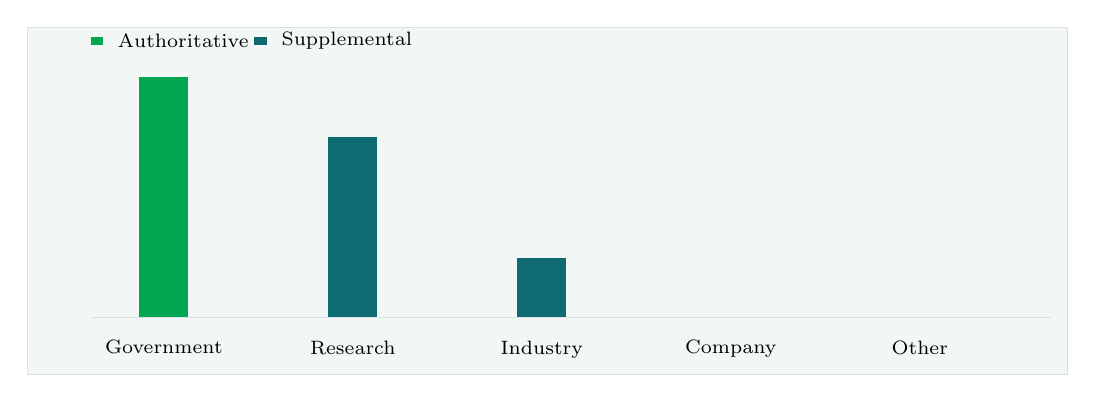
\begin{tikzpicture}[x=1cm,y=1cm]
\path[use as bounding box] (0,0) rectangle (13.20,4.40);
\fill[BOLight] (0,0) rectangle (13.20,4.40);
\draw[BOLine,line width=.35pt] (0,0) rectangle (13.20,4.40);
\draw[BOLine] (0.80,0.72) -- (13.00,0.72);
\fill[BOGreen] (1.42,0.72) rectangle (2.04,3.77);
\node[anchor=north,align=center,text width=2.21cm] at (1.73,0.55) {\scriptsize Government};
\fill[BOBlue] (3.82,0.72) rectangle (4.44,3.01);
\node[anchor=north,align=center,text width=2.21cm] at (4.13,0.55) {\scriptsize Research};
\fill[BOBlue] (6.22,0.72) rectangle (6.84,1.48);
\node[anchor=north,align=center,text width=2.21cm] at (6.53,0.55) {\scriptsize Industry};
\node[anchor=north,align=center,text width=2.21cm] at (8.93,0.55) {\scriptsize Company};
\node[anchor=north,align=center,text width=2.21cm] at (11.33,0.55) {\scriptsize Other};
\fill[BOGreen] (0.80,4.18) rectangle (0.96,4.28);
\node[anchor=west] at (1.02,4.23) {\scriptsize Authoritative};
\fill[BOBlue] (2.88,4.18) rectangle (3.04,4.28);
\node[anchor=west] at (3.10,4.23) {\scriptsize Supplemental};
\end{tikzpicture}\par\vspace{2pt}
\vspace{1pt}\noindent\begin{minipage}[t]{0.56\linewidth}
{\footnotesize\color{BOText} Institution type matters because CEO conclusions are stronger when public agencies, laboratories, research bodies and industry sources point in the same direction.}\par
\end{minipage}\hfill\begin{minipage}[t]{0.36\linewidth}
{\scriptsize\color{BOText}\begin{tabular}{p{31mm}>{\raggedleft\arraybackslash}p{18mm}}
\multicolumn{2}{l}{\textcolor{BOGreen}{\bfseries Visible readout}}\\[2pt]
Government & \textbf{4}\\[1pt]
Research & \textbf{3}\\[1pt]
Industry & \textbf{1}\\[1pt]
Company & \textbf{0}\\[1pt]
Other & \textbf{0}\\[1pt]
\end{tabular}}\par
\end{minipage}\par\vspace{1pt}
\vspace{4pt}{\footnotesize\color{BOText} Institution type matters because CEO conclusions are stronger when public agencies, laboratories, research bodies and industry sources point in the same direction.}\par
{\scriptsize\color{BOMuted} Sources: science.osti.gov; energy.gov; iaea.org; iter.org.}\par
\vspace{9pt}\textcolor{BOLine}{\rule{\linewidth}{0.3pt}}\vspace{8pt}
{\textcolor{BOGreen}{\scriptsize\bfseries EXHIBIT 2}}\par\vspace{4pt}
{\sffamily\fontsize{17}{21}\selectfont\color{BONavy} Source domains define where firm claims can be made}\par
{\small\color{BOText} Each bar represents a public web or document domain behind the analysis.}\par\vspace{6pt}
\noindent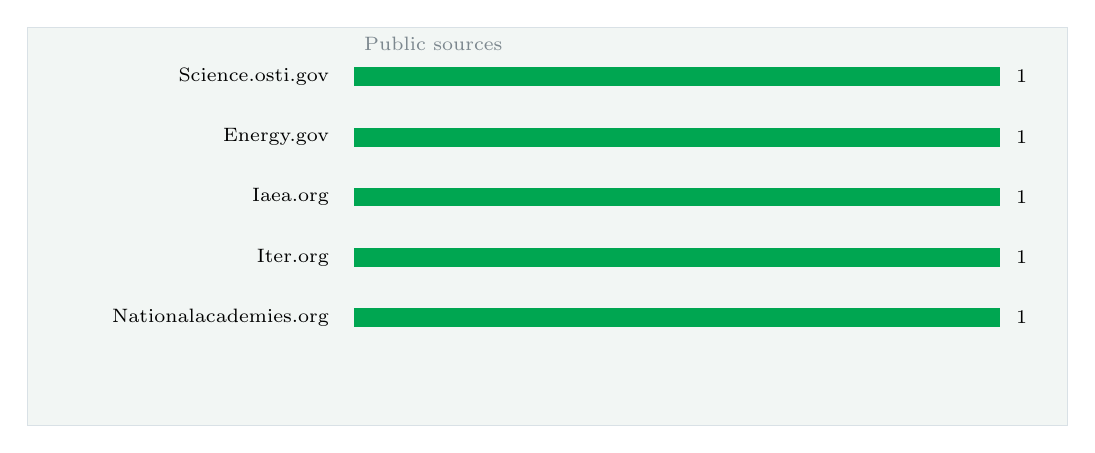
\begin{tikzpicture}[x=1cm,y=1cm]
\path[use as bounding box] (0,0) rectangle (13.20,5.05);
\fill[BOLight] (0,0) rectangle (13.20,5.05);
\draw[BOLine,line width=.35pt] (0,0) rectangle (13.20,5.05);
\node[anchor=west] at (4.15,4.85) {\scriptsize\color{BOMuted} Public sources};
\node[anchor=east,align=right,text width=3.93cm] at (3.95,4.43) {\scriptsize Science.osti.gov};
\fill[BOLight] (4.15,4.31) rectangle (12.35,4.55);
\fill[BOGreen] (4.15,4.31) rectangle (12.35,4.55);
\node[anchor=west] at (12.43,4.43) {\scriptsize 1};
\node[anchor=east,align=right,text width=3.93cm] at (3.95,3.66) {\scriptsize Energy.gov};
\fill[BOLight] (4.15,3.54) rectangle (12.35,3.78);
\fill[BOGreen] (4.15,3.54) rectangle (12.35,3.78);
\node[anchor=west] at (12.43,3.66) {\scriptsize 1};
\node[anchor=east,align=right,text width=3.93cm] at (3.95,2.90) {\scriptsize Iaea.org};
\fill[BOLight] (4.15,2.78) rectangle (12.35,3.02);
\fill[BOGreen] (4.15,2.78) rectangle (12.35,3.02);
\node[anchor=west] at (12.43,2.90) {\scriptsize 1};
\node[anchor=east,align=right,text width=3.93cm] at (3.95,2.13) {\scriptsize Iter.org};
\fill[BOLight] (4.15,2.01) rectangle (12.35,2.25);
\fill[BOGreen] (4.15,2.01) rectangle (12.35,2.25);
\node[anchor=west] at (12.43,2.13) {\scriptsize 1};
\node[anchor=east,align=right,text width=3.93cm] at (3.95,1.37) {\scriptsize Nationalacademies.org};
\fill[BOLight] (4.15,1.25) rectangle (12.35,1.49);
\fill[BOGreen] (4.15,1.25) rectangle (12.35,1.49);
\node[anchor=west] at (12.43,1.37) {\scriptsize 1};
\end{tikzpicture}\par\vspace{2pt}
\vspace{1pt}\noindent\begin{minipage}[t]{0.56\linewidth}
{\footnotesize\color{BOText} A narrow domain base limits how far the narrative should generalize across markets, technologies or regulatory settings.}\par
\end{minipage}\hfill\begin{minipage}[t]{0.36\linewidth}
{\scriptsize\color{BOText}\begin{tabular}{p{31mm}>{\raggedleft\arraybackslash}p{18mm}}
\multicolumn{2}{l}{\textcolor{BOGreen}{\bfseries Visible readout}}\\[2pt]
Science.osti.gov & \textbf{1}\\[1pt]
Energy.gov & \textbf{1}\\[1pt]
Iaea.org & \textbf{1}\\[1pt]
Iter.org & \textbf{1}\\[1pt]
Nationalacademies.org & \textbf{1}\\[1pt]
\end{tabular}}\par
\end{minipage}\par\vspace{1pt}
\vspace{4pt}{\footnotesize\color{BOText} A narrow domain base limits how far the narrative should generalize across markets, technologies or regulatory settings.}\par
{\scriptsize\color{BOMuted} Sources: science.osti.gov; energy.gov; iaea.org; iter.org.}\par

\clearpage
{\textcolor{BOGreen}{\scriptsize\bfseries EXHIBIT 3}}\par\vspace{4pt}
{\sffamily\fontsize{17}{21}\selectfont\color{BONavy} Evidence breadth depends on adding independent domains}\par
{\small\color{BOText} Cumulative public sources and unique domains across the evidence base.}\par\vspace{6pt}
\noindent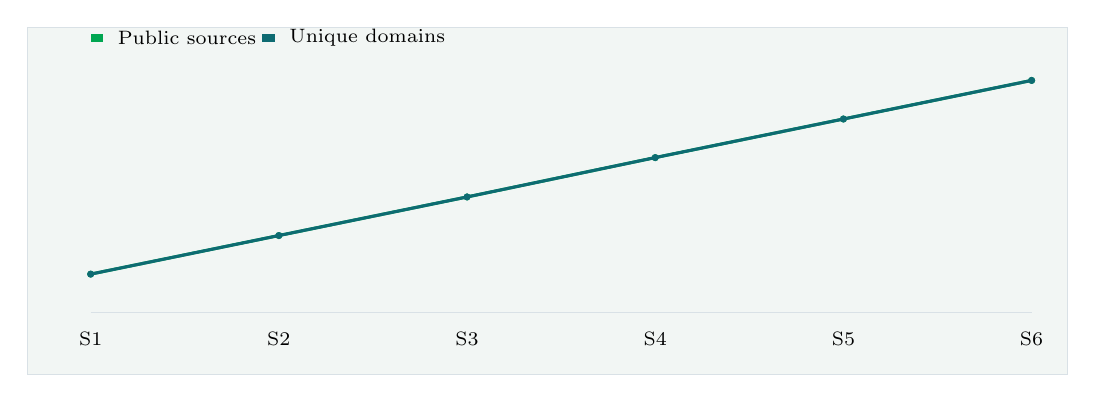
\begin{tikzpicture}[x=1cm,y=1cm]
\path[use as bounding box] (0,0) rectangle (13.20,4.40);
\fill[BOLight] (0,0) rectangle (13.20,4.40);
\draw[BOLine,line width=.35pt] (0,0) rectangle (13.20,4.40);
\draw[BOLine] (0.80,0.78) -- (12.75,0.78);
\draw[BOGreen,line width=1.1pt] (0.80,1.27) -- (3.19,1.76) -- (5.58,2.25) -- (7.97,2.75) -- (10.36,3.24) -- (12.75,3.73);
\fill[BOGreen] (0.80,1.27) circle (.045);
\fill[BOGreen] (3.19,1.76) circle (.045);
\fill[BOGreen] (5.58,2.25) circle (.045);
\fill[BOGreen] (7.97,2.75) circle (.045);
\fill[BOGreen] (10.36,3.24) circle (.045);
\fill[BOGreen] (12.75,3.73) circle (.045);
\draw[BOBlue,line width=1.1pt] (0.80,1.27) -- (3.19,1.76) -- (5.58,2.25) -- (7.97,2.75) -- (10.36,3.24) -- (12.75,3.73);
\fill[BOBlue] (0.80,1.27) circle (.045);
\fill[BOBlue] (3.19,1.76) circle (.045);
\fill[BOBlue] (5.58,2.25) circle (.045);
\fill[BOBlue] (7.97,2.75) circle (.045);
\fill[BOBlue] (10.36,3.24) circle (.045);
\fill[BOBlue] (12.75,3.73) circle (.045);
\node[anchor=north,align=center,text width=1.8cm] at (0.80,0.66) {\scriptsize S1};
\node[anchor=north,align=center,text width=1.8cm] at (3.19,0.66) {\scriptsize S2};
\node[anchor=north,align=center,text width=1.8cm] at (5.58,0.66) {\scriptsize S3};
\node[anchor=north,align=center,text width=1.8cm] at (7.97,0.66) {\scriptsize S4};
\node[anchor=north,align=center,text width=1.8cm] at (10.36,0.66) {\scriptsize S5};
\node[anchor=north,align=center,text width=1.8cm] at (12.75,0.66) {\scriptsize S6};
\fill[BOGreen] (0.80,4.22) rectangle (0.96,4.32);
\node[anchor=west] at (1.02,4.27) {\scriptsize Public sources};
\fill[BOBlue] (2.98,4.22) rectangle (3.14,4.32);
\node[anchor=west] at (3.20,4.27) {\scriptsize Unique domains};
\end{tikzpicture}\par\vspace{2pt}
\vspace{1pt}\noindent\begin{minipage}[t]{0.56\linewidth}
{\footnotesize\color{BOText} A stronger fact base adds both more sources and more independent domains, rather than repeating one institution.}\par
\end{minipage}\hfill\begin{minipage}[t]{0.36\linewidth}
{\scriptsize\color{BOText}\begin{tabular}{p{31mm}>{\raggedleft\arraybackslash}p{18mm}}
\multicolumn{2}{l}{\textcolor{BOGreen}{\bfseries Visible readout}}\\[2pt]
S1 & \textbf{2}\\[1pt]
S2 & \textbf{4}\\[1pt]
S3 & \textbf{6}\\[1pt]
S4 & \textbf{8}\\[1pt]
S5 & \textbf{10}\\[1pt]
\end{tabular}}\par
\end{minipage}\par\vspace{1pt}
\vspace{4pt}{\footnotesize\color{BOText} A stronger fact base adds both more sources and more independent domains, rather than repeating one institution.}\par
{\scriptsize\color{BOMuted} Sources: science.osti.gov; energy.gov; iaea.org; iter.org.}\par
\vspace{9pt}\textcolor{BOLine}{\rule{\linewidth}{0.3pt}}\vspace{8pt}
{\textcolor{BOGreen}{\scriptsize\bfseries EXHIBIT 4}}\par\vspace{4pt}
{\sffamily\fontsize{17}{21}\selectfont\color{BONavy} Public facts cluster by technical, policy and commercial themes}\par
{\small\color{BOText} Mention counts across public facts, dated facts and numeric facts.}\par\vspace{6pt}
\noindent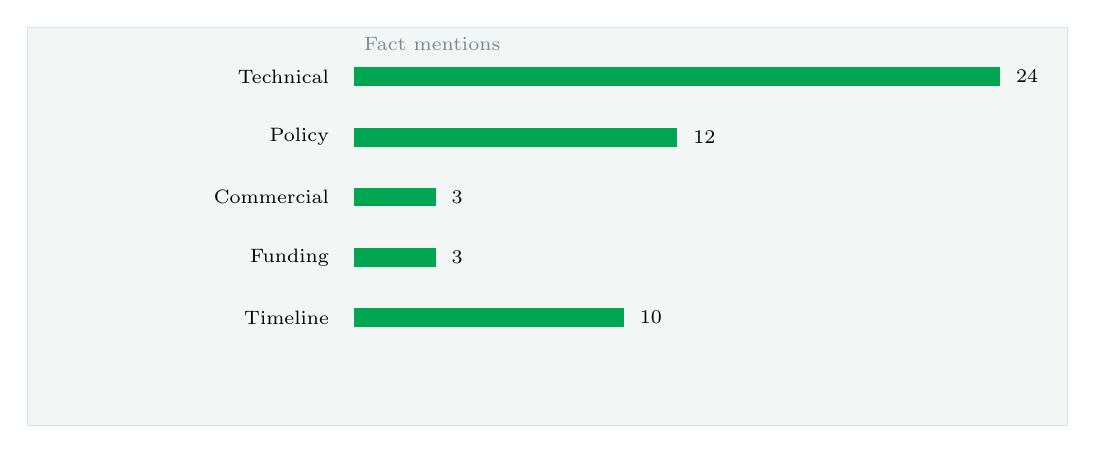
\begin{tikzpicture}[x=1cm,y=1cm]
\path[use as bounding box] (0,0) rectangle (13.20,5.05);
\fill[BOLight] (0,0) rectangle (13.20,5.05);
\draw[BOLine,line width=.35pt] (0,0) rectangle (13.20,5.05);
\node[anchor=west] at (4.15,4.85) {\scriptsize\color{BOMuted} Fact mentions};
\node[anchor=east,align=right,text width=3.93cm] at (3.95,4.43) {\scriptsize Technical};
\fill[BOLight] (4.15,4.31) rectangle (12.35,4.55);
\fill[BOGreen] (4.15,4.31) rectangle (12.35,4.55);
\node[anchor=west] at (12.43,4.43) {\scriptsize 24};
\node[anchor=east,align=right,text width=3.93cm] at (3.95,3.66) {\scriptsize Policy};
\fill[BOLight] (4.15,3.54) rectangle (12.35,3.78);
\fill[BOGreen] (4.15,3.54) rectangle (8.25,3.78);
\node[anchor=west] at (8.33,3.66) {\scriptsize 12};
\node[anchor=east,align=right,text width=3.93cm] at (3.95,2.90) {\scriptsize Commercial};
\fill[BOLight] (4.15,2.78) rectangle (12.35,3.02);
\fill[BOGreen] (4.15,2.78) rectangle (5.18,3.02);
\node[anchor=west] at (5.26,2.90) {\scriptsize 3};
\node[anchor=east,align=right,text width=3.93cm] at (3.95,2.13) {\scriptsize Funding};
\fill[BOLight] (4.15,2.01) rectangle (12.35,2.25);
\fill[BOGreen] (4.15,2.01) rectangle (5.18,2.25);
\node[anchor=west] at (5.26,2.13) {\scriptsize 3};
\node[anchor=east,align=right,text width=3.93cm] at (3.95,1.37) {\scriptsize Timeline};
\fill[BOLight] (4.15,1.25) rectangle (12.35,1.49);
\fill[BOGreen] (4.15,1.25) rectangle (7.57,1.49);
\node[anchor=west] at (7.65,1.37) {\scriptsize 10};
\end{tikzpicture}\par\vspace{2pt}
\vspace{1pt}\noindent\begin{minipage}[t]{0.56\linewidth}
{\footnotesize\color{BOText} The mix indicates whether the public record is led by technical milestones, policy institutions or commercial proof.}\par
\end{minipage}\hfill\begin{minipage}[t]{0.36\linewidth}
{\scriptsize\color{BOText}\begin{tabular}{p{31mm}>{\raggedleft\arraybackslash}p{18mm}}
\multicolumn{2}{l}{\textcolor{BOGreen}{\bfseries Visible readout}}\\[2pt]
Technical & \textbf{24}\\[1pt]
Policy & \textbf{12}\\[1pt]
Commercial & \textbf{3}\\[1pt]
Funding & \textbf{3}\\[1pt]
Timeline & \textbf{10}\\[1pt]
\end{tabular}}\par
\end{minipage}\par\vspace{1pt}
\vspace{4pt}{\footnotesize\color{BOText} The mix indicates whether the public record is led by technical milestones, policy institutions or commercial proof.}\par
{\scriptsize\color{BOMuted} Sources: science.osti.gov; energy.gov; iaea.org; iter.org.}\par

\clearpage
\label{chap:1}
\noindent\begin{tikzpicture}
\path[use as bounding box] (0,0) rectangle (\linewidth,54mm);
\clip (0,0) rectangle (\linewidth,54mm);
\node[anchor=north west,inner sep=0] at (0,54mm) {
\includegraphics[width=\linewidth]{assets/image-1.png}};
\end{tikzpicture}
\vspace{0pt}
\noindent
\begin{tikzpicture}
\fill[BOGreen] (0,0) rectangle (96mm,1.2pt);
\end{tikzpicture}\par\vspace{8pt}
{\Large\sffamily\bfseries\color{BONavy} Fusion Commercialization Is Likely Post-2035 with Significant Uncertainty}\par\vspace{4pt}
{\sffamily\fontsize{15}{20}\selectfont\color{BOGreen} The commercialization timeline for fusion energy is highly uncertain, with private ventures targeting 2028-2032 pilot plants but public projects like ITER facing delays to the 2030s. Executives should plan for a 2035-2050 window and stage investments based on key milestones.}\par\vspace{9pt}
\begin{multicols}{2}
{\small The path to commercial fusion energy is defined by a series of ambitious public and private projects, each targeting key milestones. The most prominent public project, ITER, is an international tokamak under construction in France, with first plasma expected in the 2030s and full deuterium-tritium operation later that decade. ITER is designed to produce 500 MW of fusion power for 400 seconds, demonstrating the physics and engineering of a burning plasma. However, ITER has faced repeated delays and cost overruns, with the original 2020 first plasma now pushed to the 2030s. The next step, DEMO, is not expected until the 2040s at the earliest.}\par
{\small Private ventures are pursuing faster timelines. Commonwealth Fusion Systems (CFS), a spinout from MIT, is building SPARC, a compact tokamak using high-temperature superconducting magnets. SPARC aims to achieve net energy gain (Q>1) by 2025-2026, with a commercial pilot plant targeted for the early 2030s. Helion Energy, backed by Sam Altman, plans to demonstrate a 50 MW commercial reactor by 2028 using a field-reversed configuration. TAE Technologies is pursuing a linear design with a goal of commercial power by 2030. These private companies have raised over \$5 billion collectively, according to the Fusion Industry Association.}\par
{\small The 2022 achievement of fusion ignition at Lawrence Livermore National Laboratory (LLNL) was a historic scientific milestone, demonstrating that a controlled fusion reaction can produce more energy than the laser energy used to drive it. However, this was a single-shot experiment using inertial confinement, not a sustained power source. The National Ignition Facility (NIF) is not designed for continuous operation, and significant engineering challenges remain to convert this approach into a commercial power plant.}\par
{\small Key technical challenges include sustaining a burning plasma for extended periods, developing materials that can withstand high neutron fluxes, breeding tritium fuel, and designing efficient power conversion systems. The DOE\BOApos{}s Milestone-Based Fusion Development Program is a public-private partnership aimed at resolving these risks, with awards to eight companies including CFS, Helion, and TAE. The program provides funding contingent on achieving specific technical milestones, reducing the financial burden on private companies.}\par
{\small Realistic commercialization timelines vary widely. Optimistic projections from private companies suggest pilot plants by 2028-2032, but independent assessments, including the National Academies study, indicate that commercial fusion electricity is unlikely before 2040-2050. The Fusion Industry Association\BOApos{}s 2024 report notes that most companies expect to deliver power to the grid in the 2030s, but these projections are subject to significant technical and regulatory risks.}\par
{\small For leadership teams, the key takeaway is that fusion is not imminent but is progressing faster than many expect. The next five years will be critical: if SPARC achieves net energy gain, it will validate the compact tokamak approach and attract further investment. If ITER faces further delays, it may shift focus to private alternatives. Companies should monitor these milestones closely and be prepared to adjust strategies accordingly.}\par
\end{multicols}
\label{chap:1:end}

\clearpage
{\textcolor{BOGreen}{\scriptsize\bfseries EXHIBIT 5}}\par\vspace{4pt}
{\sffamily\fontsize{17}{21}\selectfont\color{BONavy} Dated facts anchor the chronology where public text permits it}\par
{\small\color{BOText} Year mentions found in public facts and source references.}\par\vspace{6pt}
\noindent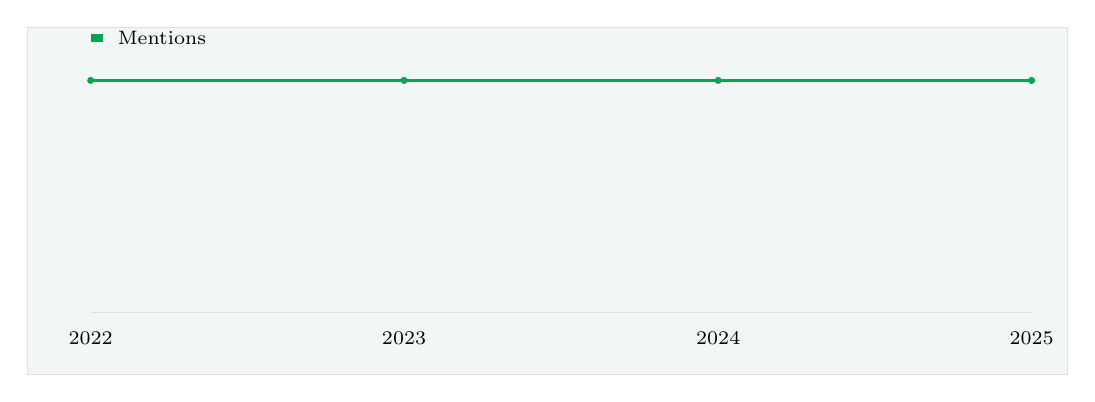
\begin{tikzpicture}[x=1cm,y=1cm]
\path[use as bounding box] (0,0) rectangle (13.20,4.40);
\fill[BOLight] (0,0) rectangle (13.20,4.40);
\draw[BOLine,line width=.35pt] (0,0) rectangle (13.20,4.40);
\draw[BOLine] (0.80,0.78) -- (12.75,0.78);
\draw[BOGreen,line width=1.1pt] (0.80,3.73) -- (4.78,3.73) -- (8.77,3.73) -- (12.75,3.73);
\fill[BOGreen] (0.80,3.73) circle (.045);
\fill[BOGreen] (4.78,3.73) circle (.045);
\fill[BOGreen] (8.77,3.73) circle (.045);
\fill[BOGreen] (12.75,3.73) circle (.045);
\node[anchor=north,align=center,text width=1.8cm] at (0.80,0.66) {\scriptsize 2022};
\node[anchor=north,align=center,text width=1.8cm] at (4.78,0.66) {\scriptsize 2023};
\node[anchor=north,align=center,text width=1.8cm] at (8.77,0.66) {\scriptsize 2024};
\node[anchor=north,align=center,text width=1.8cm] at (12.75,0.66) {\scriptsize 2025};
\fill[BOGreen] (0.80,4.22) rectangle (0.96,4.32);
\node[anchor=west] at (1.02,4.27) {\scriptsize Mentions};
\end{tikzpicture}\par\vspace{2pt}
\vspace{1pt}\noindent\begin{minipage}[t]{0.56\linewidth}
{\footnotesize\color{BOText} Timeline claims are stronger when they can be tied to explicit years rather than broad commercialization language.}\par
\end{minipage}\hfill\begin{minipage}[t]{0.36\linewidth}
{\scriptsize\color{BOText}\begin{tabular}{p{31mm}>{\raggedleft\arraybackslash}p{18mm}}
\multicolumn{2}{l}{\textcolor{BOGreen}{\bfseries Visible readout}}\\[2pt]
2022 & \textbf{1}\\[1pt]
2023 & \textbf{1}\\[1pt]
2024 & \textbf{1}\\[1pt]
2025 & \textbf{1}\\[1pt]
\end{tabular}}\par
\end{minipage}\par\vspace{1pt}
\vspace{4pt}{\footnotesize\color{BOText} Timeline claims are stronger when they can be tied to explicit years rather than broad commercialization language.}\par
{\scriptsize\color{BOMuted} Sources: science.osti.gov; energy.gov; iaea.org; iter.org.}\par
\vspace{9pt}\textcolor{BOLine}{\rule{\linewidth}{0.3pt}}\vspace{8pt}
{\textcolor{BOGreen}{\scriptsize\bfseries EXHIBIT 6}}\par\vspace{4pt}
{\sffamily\fontsize{17}{21}\selectfont\color{BONavy} Source type mix separates full pages from thin snippets}\par
{\small\color{BOText} Public sources by content form and authority flag.}\par\vspace{6pt}
\noindent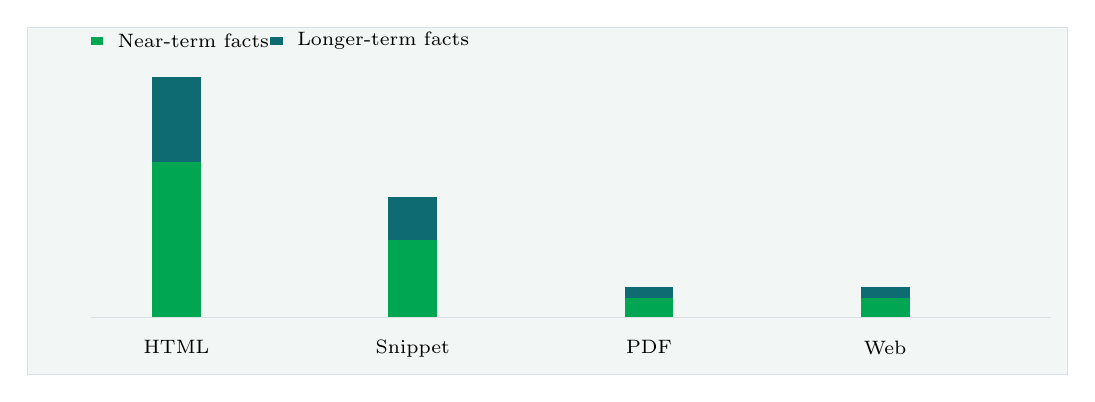
\begin{tikzpicture}[x=1cm,y=1cm]
\path[use as bounding box] (0,0) rectangle (13.20,4.40);
\fill[BOLight] (0,0) rectangle (13.20,4.40);
\draw[BOLine,line width=.35pt] (0,0) rectangle (13.20,4.40);
\draw[BOLine] (0.80,0.72) -- (13.00,0.72);
\fill[BOGreen] (1.58,0.72) rectangle (2.20,2.69);
\fill[BOBlue] (1.58,2.69) rectangle (2.20,3.77);
\node[anchor=north,align=center,text width=2.76cm] at (1.89,0.55) {\scriptsize HTML};
\fill[BOGreen] (4.58,0.72) rectangle (5.20,1.70);
\fill[BOBlue] (4.58,1.70) rectangle (5.20,2.25);
\node[anchor=north,align=center,text width=2.76cm] at (4.89,0.55) {\scriptsize Snippet};
\fill[BOGreen] (7.58,0.72) rectangle (8.20,0.97);
\fill[BOBlue] (7.58,0.97) rectangle (8.20,1.11);
\node[anchor=north,align=center,text width=2.76cm] at (7.89,0.55) {\scriptsize PDF};
\fill[BOGreen] (10.58,0.72) rectangle (11.20,0.97);
\fill[BOBlue] (10.58,0.97) rectangle (11.20,1.11);
\node[anchor=north,align=center,text width=2.76cm] at (10.89,0.55) {\scriptsize Web};
\fill[BOGreen] (0.80,4.18) rectangle (0.96,4.28);
\node[anchor=west] at (1.02,4.23) {\scriptsize Near-term facts};
\fill[BOBlue] (3.08,4.18) rectangle (3.24,4.28);
\node[anchor=west] at (3.30,4.23) {\scriptsize Longer-term facts};
\end{tikzpicture}\par\vspace{2pt}
\vspace{1pt}\noindent\begin{minipage}[t]{0.56\linewidth}
{\footnotesize\color{BOText} Pages and PDFs with extractable body text can support richer prose than snippets that carry only limited context.}\par
\end{minipage}\hfill\begin{minipage}[t]{0.36\linewidth}
{\scriptsize\color{BOText}\begin{tabular}{p{31mm}>{\raggedleft\arraybackslash}p{18mm}}
\multicolumn{2}{l}{\textcolor{BOGreen}{\bfseries Visible readout}}\\[2pt]
HTML & \textbf{37.2}\\[1pt]
Snippet & \textbf{18.6}\\[1pt]
PDF & \textbf{4.7}\\[1pt]
Web & \textbf{4.7}\\[1pt]
\end{tabular}}\par
\end{minipage}\par\vspace{1pt}
\vspace{4pt}{\footnotesize\color{BOText} Pages and PDFs with extractable body text can support richer prose than snippets that carry only limited context.}\par
{\scriptsize\color{BOMuted} Sources: science.osti.gov; energy.gov; iaea.org; iter.org.}\par

\clearpage
\label{chap:2}
\noindent\begin{tikzpicture}
\path[use as bounding box] (0,0) rectangle (\linewidth,54mm);
\clip (0,0) rectangle (\linewidth,54mm);
\node[anchor=north west,inner sep=0] at (0,54mm) {
\includegraphics[width=\linewidth]{assets/image-2.png}};
\end{tikzpicture}
\vspace{0pt}
\noindent
\begin{tikzpicture}
\fill[BOGreen] (0,0) rectangle (96mm,1.2pt);
\end{tikzpicture}\par\vspace{8pt}
{\Large\sffamily\bfseries\color{BONavy} Fusion Faces High Cost Hurdles but Could Be Competitive in Baseload Markets}\par\vspace{4pt}
{\sffamily\fontsize{15}{20}\selectfont\color{BOGreen} Fusion LCOE is projected at \$50-100/MWh by 2050, higher than current renewables but competitive for baseload applications. Executives should view fusion as a complement to renewables, not a replacement, and focus on high-value markets.}\par\vspace{9pt}
\begin{multicols}{2}
{\small The economic viability of fusion energy depends on its levelized cost of energy (LCOE) relative to other sources. Current estimates from the DOE and industry analysts project fusion LCOE in the range of \$50-100/MWh by 2050, assuming successful commercialization. For comparison, solar and wind with storage are already at \$30-60/MWh in many markets, and costs continue to decline. Natural gas combined cycle plants have LCOE around \$40-80/MWh, while nuclear fission is \$100-150/MWh for new builds.}\par
{\small Fusion\BOApos{}s potential advantage lies in its high capacity factor (90\%+), low fuel cost (deuterium from seawater is virtually free), and lack of carbon emissions or long-lived radioactive waste. This makes it an attractive option for baseload power, especially in regions with limited renewable resources or high land costs. However, the capital cost of a first-of-a-kind fusion plant is estimated at \$5-10 billion, with significant uncertainty. Learning curve effects could reduce costs by 30-50\% for subsequent plants, similar to the experience with nuclear fission.}\par
{\small Financing fusion plants will be challenging due to the high upfront capital and perceived technology risk. Government loan guarantees, power purchase agreements (PPAs), and carbon pricing could help de-risk investments. The DOE\BOApos{}s Loan Programs Office has already expressed interest in supporting fusion projects. In the UK, the government has committed £220 million to the STEP fusion program, aiming for a prototype plant by 2040.}\par
{\small Regulatory hurdles are another cost factor. Fusion plants will likely require licensing similar to nuclear fission, but the regulatory framework is still undeveloped. The U.S. Nuclear Regulatory Commission (NRC) is working on a risk-informed, performance-based framework for fusion, but this may take years to finalize. In the interim, fusion developers may face lengthy and uncertain licensing processes, adding to costs and timelines.}\par
{\small Market demand for fusion will depend on the pace of decarbonization and the competitiveness of alternatives. In a high-decarbonization scenario, demand for clean baseload power could be strong, especially if renewables face integration challenges. Fusion could also serve niche markets such as industrial heat (e.g., steel, cement) and hydrogen production, where high temperatures are required. The global hydrogen market is projected to grow to \$200 billion by 2050, and fusion could provide low-cost, carbon-free hydrogen via high-temperature electrolysis.}\par
{\small In capital terms, the key takeaway is that fusion is unlikely to be the cheapest electricity source in the 2030s, but it could be competitive in specific applications and markets. Companies should model fusion as a potential complement to renewables, not a replacement. Strategic investments should target high-value applications where fusion\BOApos{}s baseload capability and low fuel cost provide a clear advantage.}\par
\end{multicols}
\label{chap:2:end}

\clearpage
{\textcolor{BOGreen}{\scriptsize\bfseries EXHIBIT 7}}\par\vspace{4pt}
{\sffamily\fontsize{17}{21}\selectfont\color{BONavy} Business relevance depends on numbers, dates and commercial proof}\par
{\small\color{BOText} Numeric, dated and commercial references across the main narrative.}\par\vspace{6pt}
\noindent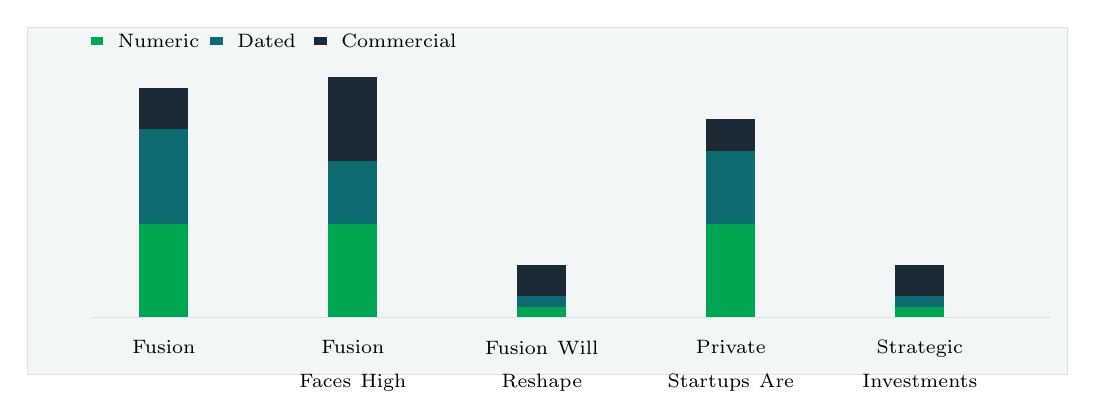
\begin{tikzpicture}[x=1cm,y=1cm]
\path[use as bounding box] (0,0) rectangle (13.20,4.40);
\fill[BOLight] (0,0) rectangle (13.20,4.40);
\draw[BOLine,line width=.35pt] (0,0) rectangle (13.20,4.40);
\draw[BOLine] (0.80,0.72) -- (13.00,0.72);
\fill[BOGreen] (1.42,0.72) rectangle (2.04,1.91);
\fill[BOBlue] (1.42,1.91) rectangle (2.04,3.11);
\fill[BONavy] (1.42,3.11) rectangle (2.04,3.64);
\node[anchor=north,align=center,text width=2.21cm] at (1.73,0.55) {\scriptsize Fusion};
\fill[BOGreen] (3.82,0.72) rectangle (4.44,1.91);
\fill[BOBlue] (3.82,1.91) rectangle (4.44,2.71);
\fill[BONavy] (3.82,2.71) rectangle (4.44,3.77);
\node[anchor=north,align=center,text width=2.21cm] at (4.13,0.55) {\scriptsize Fusion Faces High};
\fill[BOGreen] (6.22,0.72) rectangle (6.84,0.85);
\fill[BOBlue] (6.22,0.85) rectangle (6.84,0.99);
\fill[BONavy] (6.22,0.99) rectangle (6.84,1.38);
\node[anchor=north,align=center,text width=2.21cm] at (6.53,0.55) {\scriptsize Fusion Will Reshape};
\fill[BOGreen] (8.62,0.72) rectangle (9.24,1.91);
\fill[BOBlue] (8.62,1.91) rectangle (9.24,2.84);
\fill[BONavy] (8.62,2.84) rectangle (9.24,3.24);
\node[anchor=north,align=center,text width=2.21cm] at (8.93,0.55) {\scriptsize Private Startups Are};
\fill[BOGreen] (11.02,0.72) rectangle (11.64,0.85);
\fill[BOBlue] (11.02,0.85) rectangle (11.64,0.99);
\fill[BONavy] (11.02,0.99) rectangle (11.64,1.38);
\node[anchor=north,align=center,text width=2.21cm] at (11.33,0.55) {\scriptsize Strategic Investments};
\fill[BOGreen] (0.80,4.18) rectangle (0.96,4.28);
\node[anchor=west] at (1.02,4.23) {\scriptsize Numeric};
\fill[BOBlue] (2.32,4.18) rectangle (2.48,4.28);
\node[anchor=west] at (2.54,4.23) {\scriptsize Dated};
\fill[BONavy] (3.64,4.18) rectangle (3.80,4.28);
\node[anchor=west] at (3.86,4.23) {\scriptsize Commercial};
\end{tikzpicture}\par\vspace{2pt}
\vspace{1pt}\noindent\begin{minipage}[t]{0.56\linewidth}
{\footnotesize\color{BOText} A board reader needs later pages to carry the same factual weight as the opening argument, especially around numbers and dated milestones.}\par
\end{minipage}\hfill\begin{minipage}[t]{0.36\linewidth}
{\scriptsize\color{BOText}\begin{tabular}{p{31mm}>{\raggedleft\arraybackslash}p{18mm}}
\multicolumn{2}{l}{\textcolor{BOGreen}{\bfseries Visible readout}}\\[2pt]
Fusion & \textbf{22}\\[1pt]
Fusion Faces High Cost & \textbf{23}\\[1pt]
Fusion Will Reshape & \textbf{5}\\[1pt]
Private Startups Are & \textbf{19}\\[1pt]
Strategic Investments & \textbf{5}\\[1pt]
\end{tabular}}\par
\end{minipage}\par\vspace{1pt}
\vspace{4pt}{\footnotesize\color{BOText} A board reader needs later pages to carry the same factual weight as the opening argument, especially around numbers and dated milestones.}\par
{\scriptsize\color{BOMuted} Sources: public references and report analysis.}\par
\vspace{9pt}\textcolor{BOLine}{\rule{\linewidth}{0.3pt}}\vspace{8pt}
{\textcolor{BOGreen}{\scriptsize\bfseries EXHIBIT 8}}\par\vspace{4pt}
{\sffamily\fontsize{17}{21}\selectfont\color{BONavy} Evidence support differs by business question}\par
{\small\color{BOText} A compact support matrix for the main executive questions.}\par\vspace{6pt}
\noindent\fcolorbox{BOLine}{BOLight}{\begin{minipage}{0.96\linewidth}\vspace{4pt}{\scriptsize\begin{tabular}{p{38mm}>{\centering\arraybackslash}p{21mm}>{\centering\arraybackslash}p{21mm}>{\centering\arraybackslash}p{21mm}>{\centering\arraybackslash}p{21mm}}
 & {\bfseries Sources} & {\bfseries Numbers} & {\bfseries Dates} & {\bfseries Business tie} \\
\hline
{\bfseries Fusion Commercialization Is.} & \colorbox{BOGreen}{\textcolor{white}{\strut\hspace{5pt}4\hspace{5pt}}} & \colorbox{BOGreen}{\textcolor{white}{\strut\hspace{5pt}5\hspace{5pt}}} & \colorbox{BOGreen}{\textcolor{white}{\strut\hspace{5pt}5\hspace{5pt}}} & \colorbox{BOGreen}{\textcolor{white}{\strut\hspace{5pt}4\hspace{5pt}}} \\
{\bfseries Fusion Faces High Cost Hurd.} & \colorbox{BOGreen}{\textcolor{white}{\strut\hspace{5pt}4\hspace{5pt}}} & \colorbox{BOGreen}{\textcolor{white}{\strut\hspace{5pt}5\hspace{5pt}}} & \colorbox{BOGreen}{\textcolor{white}{\strut\hspace{5pt}5\hspace{5pt}}} & \colorbox{BOGreen}{\textcolor{white}{\strut\hspace{5pt}5\hspace{5pt}}} \\
{\bfseries Fusion Will Reshape Energy.} & \colorbox{BOGreen}{\textcolor{white}{\strut\hspace{5pt}4\hspace{5pt}}} & \colorbox{BOLight}{\textcolor{BOText}{\strut\hspace{5pt}1\hspace{5pt}}} & \colorbox{BOLight}{\textcolor{BOText}{\strut\hspace{5pt}1\hspace{5pt}}} & \colorbox{BOBlue}{\textcolor{white}{\strut\hspace{5pt}3\hspace{5pt}}} \\
{\bfseries Private Startups Are Accele.} & \colorbox{BOGreen}{\textcolor{white}{\strut\hspace{5pt}4\hspace{5pt}}} & \colorbox{BOGreen}{\textcolor{white}{\strut\hspace{5pt}5\hspace{5pt}}} & \colorbox{BOGreen}{\textcolor{white}{\strut\hspace{5pt}5\hspace{5pt}}} & \colorbox{BOBlue}{\textcolor{white}{\strut\hspace{5pt}3\hspace{5pt}}} \\
{\bfseries Strategic Investments Shoul.} & \colorbox{BOGreen}{\textcolor{white}{\strut\hspace{5pt}4\hspace{5pt}}} & \colorbox{BOLight}{\textcolor{BOText}{\strut\hspace{5pt}1\hspace{5pt}}} & \colorbox{BOLight}{\textcolor{BOText}{\strut\hspace{5pt}1\hspace{5pt}}} & \colorbox{BOBlue}{\textcolor{white}{\strut\hspace{5pt}3\hspace{5pt}}} \\
\end{tabular}}\vspace{4pt}\end{minipage}}\par\vspace{2pt}
\vspace{1pt}\noindent\begin{minipage}[t]{0.56\linewidth}
{\footnotesize\color{BOText} The strongest pages connect source depth with numbers, dates and direct business implications.}\par
\end{minipage}\hfill\begin{minipage}[t]{0.36\linewidth}
{\scriptsize\color{BOText}\begin{tabular}{p{31mm}>{\raggedleft\arraybackslash}p{18mm}}
\multicolumn{2}{l}{\textcolor{BOGreen}{\bfseries Matrix readout}}\\[2pt]
Fusion & \textbf{4 / 5}\\[1pt]
Fusion Faces High & \textbf{4 / 5}\\[1pt]
Fusion Will Reshape & \textbf{4 / 1}\\[1pt]
Private Startups Are & \textbf{4 / 5}\\[1pt]
\end{tabular}}\par
\end{minipage}\par\vspace{1pt}
\vspace{4pt}{\footnotesize\color{BOText} The strongest pages connect source depth with numbers, dates and direct business implications.}\par
{\scriptsize\color{BOMuted} Sources: science.osti.gov; energy.gov; iaea.org; iter.org.}\par

\clearpage
\label{chap:3}
\noindent\begin{tikzpicture}
\path[use as bounding box] (0,0) rectangle (\linewidth,54mm);
\clip (0,0) rectangle (\linewidth,54mm);
\node[anchor=north west,inner sep=0] at (0,54mm) {
\includegraphics[width=\linewidth]{assets/image-3.png}};
\end{tikzpicture}
\vspace{0pt}
\noindent
\begin{tikzpicture}
\fill[BOGreen] (0,0) rectangle (96mm,1.2pt);
\end{tikzpicture}\par\vspace{8pt}
{\Large\sffamily\bfseries\color{BONavy} Fusion Will Reshape Energy Geopolitics, Reducing Dependence on Fossil Fuels}\par\vspace{4pt}
{\sffamily\fontsize{15}{20}\selectfont\color{BOGreen} Fusion fuel is abundant and widely distributed, potentially decoupling energy security from fossil fuel reserves. Executives should view fusion as a long-term hedge against fossil fuel price volatility and supply disruptions.}\par\vspace{9pt}
\begin{multicols}{2}
{\small Fusion energy has the potential to fundamentally alter global energy geopolitics. Unlike fossil fuels, which are concentrated in a few regions, fusion fuel (deuterium and tritium) is virtually unlimited and widely available. Deuterium can be extracted from seawater at low cost, while tritium is bred from lithium, which is also abundant. This could reduce the strategic importance of oil and gas reserves, diminishing the geopolitical leverage of fossil fuel exporters.}\par
{\small For energy-importing nations, fusion offers the prospect of energy independence. Countries like Japan, South Korea, and many European nations that currently rely on imported fossil fuels could generate their own fusion power, reducing vulnerability to supply disruptions and price spikes. The IAEA has noted that fusion could be a game-changer for energy security, particularly for nations with limited domestic energy resources.}\par
{\small However, the initial deployment of fusion is likely to be in advanced economies with strong R\&D infrastructure and regulatory frameworks. Developing countries may face barriers to adoption due to high capital costs and technical complexity. This could create a new divide between fusion-haves and have-nots, at least in the early decades. International collaboration, such as the ITER project, can help bridge this gap by sharing knowledge and reducing costs.}\par
{\small Fusion could also impact the economics of fossil fuel production. If fusion becomes a major source of electricity, demand for natural gas and coal could decline, reducing revenues for fossil fuel exporters. This could lead to economic diversification challenges for countries like Russia, Saudi Arabia, and Australia. Conversely, countries that invest early in fusion technology could gain a competitive advantage in the global energy market.}\par
{\small The geopolitical implications extend to nuclear non-proliferation. Fusion reactors do not produce weapons-grade fissile material, and the tritium fuel cycle can be designed to minimize proliferation risks. However, the technology is complex and could be misused if not properly safeguarded. The IAEA is developing safeguards for fusion, but these are not yet finalized.}\par
{\small Commercially, the key takeaway is that fusion could reshape energy markets and geopolitical dynamics over the long term. Companies should consider the implications for their supply chains, market access, and regulatory environment. Engaging with policymakers on fusion-friendly policies can help shape the future landscape.}\par
\end{multicols}
\label{chap:3:end}

\clearpage
\label{chap:4}
\noindent\begin{tikzpicture}
\path[use as bounding box] (0,0) rectangle (\linewidth,54mm);
\clip (0,0) rectangle (\linewidth,54mm);
\node[anchor=north west,inner sep=0] at (0,54mm) {
\includegraphics[width=\linewidth]{assets/image-4.png}};
\end{tikzpicture}
\vspace{0pt}
\noindent
\begin{tikzpicture}
\fill[BOGreen] (0,0) rectangle (96mm,1.2pt);
\end{tikzpicture}\par\vspace{8pt}
{\Large\sffamily\bfseries\color{BONavy} Private Startups Are Accelerating Development but Public Projects Remain Critical}\par\vspace{4pt}
{\sffamily\fontsize{15}{20}\selectfont\color{BOGreen} Private fusion companies have raised over \$5 billion and are pursuing aggressive timelines, but public projects like ITER provide essential foundational science and infrastructure. Executives should engage with both sectors.}\par\vspace{9pt}
\begin{multicols}{2}
{\small The fusion landscape has been transformed by the emergence of private startups. Since 2020, over 30 private companies have raised more than \$5 billion, according to the Fusion Industry Association. The largest private player is Commonwealth Fusion Systems (CFS), which has raised over \$2 billion from investors including Bill Gates, Breakthrough Energy Ventures, and the Government of Singapore. CFS is building SPARC, a compact tokamak that aims to achieve net energy gain by 2025-2026.}\par
{\small Other notable private companies include Helion Energy, which has raised \$500 million and plans to demonstrate a 50 MW commercial reactor by 2028 using a field-reversed configuration. TAE Technologies has raised over \$1 billion and is pursuing a linear design with a goal of commercial power by 2030. General Fusion, backed by Jeff Bezos, is developing a magnetized target fusion approach and plans a demonstration plant by 2025.}\par
{\small These private companies are driven by a sense of urgency and a willingness to take risks. They are pursuing innovative designs and faster timelines than public projects. However, they also face significant technical and financial risks. Many are still at the proof-of-concept stage and have not yet demonstrated sustained net energy gain. The Fusion Industry Association\BOApos{}s 2024 report notes that most companies expect to deliver power to the grid in the 2030s, but these projections are highly uncertain.}\par
{\small Public projects remain critical for foundational science and infrastructure. ITER, the largest fusion experiment ever built, is designed to demonstrate the physics and engineering of a burning plasma. ITER\BOApos{}s budget exceeds \$20 billion and involves seven partners: the EU, US, China, Russia, Japan, South Korea, and India. Despite delays, ITER will provide invaluable data on plasma behavior, materials, and tritium breeding that private ventures can leverage.}\par
{\small The DOE\BOApos{}s Milestone-Based Fusion Development Program is a public-private partnership that provides funding to private companies contingent on achieving technical milestones. This program reduces the financial burden on startups and helps de-risk their technologies. The DOE has awarded \$50 million to eight companies, including CFS, Helion, and TAE, with additional funding available for later stages.}\par
{\small Regulatory frameworks are still undeveloped for fusion. The U.S. Nuclear Regulatory Commission (NRC) is working on a risk-informed, performance-based framework, but this may take years to finalize. In the UK, the government has established a regulatory framework for fusion that treats it separately from nuclear fission, which could serve as a model for other countries. The lack of regulatory clarity is a major risk for fusion developers and investors.}\par
\end{multicols}
\label{chap:4:end}

\clearpage
{\textcolor{BOGreen}{\scriptsize\bfseries EXHIBIT 9}}\par\vspace{4pt}
{\sffamily\fontsize{17}{21}\selectfont\color{BONavy} Domain map separates institutional authority from factual detail}\par
{\small\color{BOText} Each point is a public domain positioned by authority and available factual detail.}\par\vspace{6pt}
\noindent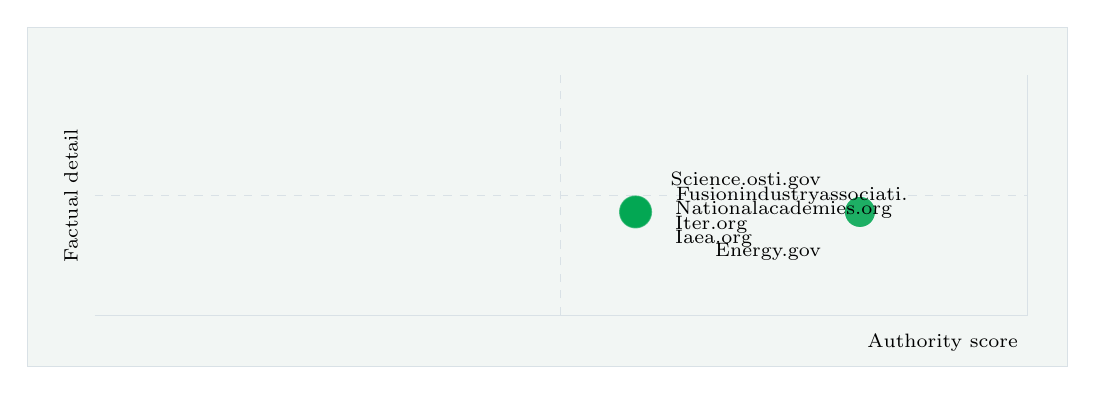
\begin{tikzpicture}[x=1cm,y=1cm]
\path[use as bounding box] (0,0) rectangle (13.20,4.30);
\fill[BOLight] (0,0) rectangle (13.20,4.30);
\draw[BOLine,line width=.35pt] (0,0) rectangle (13.20,4.30);
\draw[BOLine] (0.85,0.65) -- (12.70,0.65) -- (12.70,3.70);
\draw[BOLine,dashed] (0.85,2.17) -- (12.70,2.17);
\draw[BOLine,dashed] (6.77,0.65) -- (6.77,3.70);
\fill[BOGreen,opacity=.65] (10.57,1.96) circle (0.19);
\node[anchor=east,align=right,text width=2.10cm] at (10.20,2.35) {\scriptsize Science.osti.gov};
\fill[BOGreen,opacity=.65] (10.57,1.96) circle (0.19);
\node[anchor=east,align=right,text width=2.10cm] at (10.20,1.46) {\scriptsize Energy.gov};
\fill[BOGreen,opacity=.65] (7.72,1.96) circle (0.19);
\node[anchor=west,align=left,text width=2.10cm] at (8.10,1.62) {\scriptsize Iaea.org};
\fill[BOGreen,opacity=.65] (7.72,1.96) circle (0.20);
\node[anchor=west,align=left,text width=2.10cm] at (8.10,1.80) {\scriptsize Iter.org};
\fill[BOGreen,opacity=.65] (7.72,1.96) circle (0.20);
\node[anchor=west,align=left,text width=2.10cm] at (8.10,1.99) {\scriptsize Nationalacademies.org};
\fill[BOGreen,opacity=.65] (7.72,1.96) circle (0.21);
\node[anchor=west,align=left,text width=2.10cm] at (8.11,2.17) {\scriptsize Fusionindustryassociati.};
\node[anchor=north east] at (12.70,0.53) {\scriptsize Authority score};
\node[anchor=center,rotate=90] at (0.55,2.17) {\scriptsize Factual detail};
\end{tikzpicture}\par\vspace{2pt}
\vspace{1pt}\noindent\begin{minipage}[t]{0.56\linewidth}
{\footnotesize\color{BOText} Upper-right domains deserve more weight in the narrative because they combine credibility with extractable factual detail.}\par
\end{minipage}\hfill\begin{minipage}[t]{0.36\linewidth}
{\scriptsize\color{BOText}\begin{tabular}{p{31mm}>{\raggedleft\arraybackslash}p{18mm}}
\multicolumn{2}{l}{\textcolor{BOGreen}{\bfseries Position}}\\[2pt]
Science.osti.gov & \textbf{82 / 43}\\[1pt]
Energy.gov & \textbf{82 / 43}\\[1pt]
Iaea.org & \textbf{58 / 43}\\[1pt]
Iter.org & \textbf{58 / 43}\\[1pt]
Nationalacademies.org & \textbf{58 / 43}\\[1pt]
\end{tabular}}\par
\end{minipage}\par\vspace{1pt}
\vspace{4pt}{\footnotesize\color{BOText} Upper-right domains deserve more weight in the narrative because they combine credibility with extractable factual detail.}\par
{\scriptsize\color{BOMuted} Sources: science.osti.gov; energy.gov; iaea.org; iter.org.}\par
\vspace{9pt}\textcolor{BOLine}{\rule{\linewidth}{0.3pt}}\vspace{8pt}
{\textcolor{BOGreen}{\scriptsize\bfseries EXHIBIT 10}}\par\vspace{4pt}
{\sffamily\fontsize{17}{21}\selectfont\color{BONavy} Commercial quantification remains thinner than milestone evidence}\par
{\small\color{BOText} Numeric facts are grouped by the type of decision they can support.}\par\vspace{6pt}
\noindent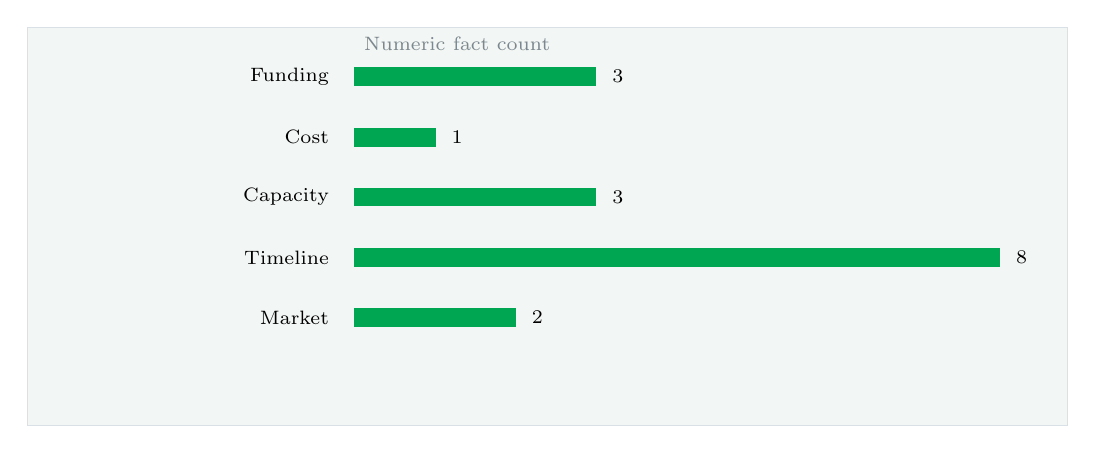
\begin{tikzpicture}[x=1cm,y=1cm]
\path[use as bounding box] (0,0) rectangle (13.20,5.05);
\fill[BOLight] (0,0) rectangle (13.20,5.05);
\draw[BOLine,line width=.35pt] (0,0) rectangle (13.20,5.05);
\node[anchor=west] at (4.15,4.85) {\scriptsize\color{BOMuted} Numeric fact count};
\node[anchor=east,align=right,text width=3.93cm] at (3.95,4.43) {\scriptsize Funding};
\fill[BOLight] (4.15,4.31) rectangle (12.35,4.55);
\fill[BOGreen] (4.15,4.31) rectangle (7.22,4.55);
\node[anchor=west] at (7.30,4.43) {\scriptsize 3};
\node[anchor=east,align=right,text width=3.93cm] at (3.95,3.66) {\scriptsize Cost};
\fill[BOLight] (4.15,3.54) rectangle (12.35,3.78);
\fill[BOGreen] (4.15,3.54) rectangle (5.18,3.78);
\node[anchor=west] at (5.26,3.66) {\scriptsize 1};
\node[anchor=east,align=right,text width=3.93cm] at (3.95,2.90) {\scriptsize Capacity};
\fill[BOLight] (4.15,2.78) rectangle (12.35,3.02);
\fill[BOGreen] (4.15,2.78) rectangle (7.22,3.02);
\node[anchor=west] at (7.30,2.90) {\scriptsize 3};
\node[anchor=east,align=right,text width=3.93cm] at (3.95,2.13) {\scriptsize Timeline};
\fill[BOLight] (4.15,2.01) rectangle (12.35,2.25);
\fill[BOGreen] (4.15,2.01) rectangle (12.35,2.25);
\node[anchor=west] at (12.43,2.13) {\scriptsize 8};
\node[anchor=east,align=right,text width=3.93cm] at (3.95,1.37) {\scriptsize Market};
\fill[BOLight] (4.15,1.25) rectangle (12.35,1.49);
\fill[BOGreen] (4.15,1.25) rectangle (6.20,1.49);
\node[anchor=west] at (6.28,1.37) {\scriptsize 2};
\end{tikzpicture}\par\vspace{2pt}
\vspace{1pt}\noindent\begin{minipage}[t]{0.56\linewidth}
{\footnotesize\color{BOText} A CEO can act faster when funding, cost, capacity and market claims are quantified instead of only described qualitatively.}\par
\end{minipage}\hfill\begin{minipage}[t]{0.36\linewidth}
{\scriptsize\color{BOText}\begin{tabular}{p{31mm}>{\raggedleft\arraybackslash}p{18mm}}
\multicolumn{2}{l}{\textcolor{BOGreen}{\bfseries Visible readout}}\\[2pt]
Funding & \textbf{3}\\[1pt]
Cost & \textbf{1}\\[1pt]
Capacity & \textbf{3}\\[1pt]
Timeline & \textbf{8}\\[1pt]
Market & \textbf{2}\\[1pt]
\end{tabular}}\par
\end{minipage}\par\vspace{1pt}
\vspace{4pt}{\footnotesize\color{BOText} A CEO can act faster when funding, cost, capacity and market claims are quantified instead of only described qualitatively.}\par
{\scriptsize\color{BOMuted} Sources: science.osti.gov; energy.gov; iaea.org; iter.org.}\par

\clearpage
\label{chap:5}
\noindent\begin{tikzpicture}
\path[use as bounding box] (0,0) rectangle (\linewidth,54mm);
\clip (0,0) rectangle (\linewidth,54mm);
\node[anchor=north west,inner sep=0] at (0,54mm) {
\includegraphics[width=\linewidth]{assets/image-5.png}};
\end{tikzpicture}
\vspace{0pt}
\noindent
\begin{tikzpicture}
\fill[BOGreen] (0,0) rectangle (96mm,1.2pt);
\end{tikzpicture}\par\vspace{8pt}
{\Large\sffamily\bfseries\color{BONavy} Strategic Investments Should Focus on Enabling Technologies and Early Partnerships}\par\vspace{4pt}
{\sffamily\fontsize{15}{20}\selectfont\color{BOGreen} Key enabling technologies include high-temperature superconductors, tritium breeding, and advanced materials. Early partnerships with fusion developers can provide preferential access to future power purchase agreements.}\par\vspace{9pt}
\begin{multicols}{2}
{\small Strategic investments in fusion should focus on enabling technologies that are critical to multiple reactor designs. High-temperature superconductors (HTS) are a key enabler for compact tokamaks like SPARC, allowing stronger magnetic fields in a smaller device. HTS technology is also used in other applications such as MRI machines and particle accelerators, providing a diversified market. Companies like SuperPower (a subsidiary of Furukawa Electric) and AMSC are leading HTS manufacturers.}\par
{\small Tritium breeding is another critical technology. Fusion reactors require tritium as fuel, but tritium is scarce and must be bred from lithium in a blanket surrounding the reactor. Developing efficient tritium breeding systems is essential for commercial fusion. Several companies and research institutions are working on this, including the UK\BOApos{}s Atomic Energy Authority and the EU\BOApos{}s DEMO program.}\par
{\small Advanced materials for reactor walls and components are also needed. Fusion reactors produce high-energy neutrons that can damage materials over time. Developing materials that can withstand high neutron fluxes and high temperatures is a key challenge. Research is ongoing on materials such as tungsten, vanadium alloys, and silicon carbide composites.}\par
{\small Fusion-specific power conversion systems are another area of investment. Fusion reactors produce heat that must be converted to electricity using turbines or other systems. Efficient power conversion is critical for economic viability. Some fusion designs also produce high-temperature heat that can be used for industrial processes or hydrogen production.}\par
{\small Early partnerships with fusion developers can provide preferential access to future power purchase agreements (PPAs) or technology licenses. For example, utilities can sign memoranda of understanding with fusion developers to secure offtake agreements once commercial plants are built. This can help de-risk investments for developers and provide utilities with a competitive advantage.}\par
{\small Industry consortia such as the Fusion Industry Association (FIA) provide a platform for collaboration and advocacy. Joining the FIA can help companies shape standards, share best practices, and gain early insights into technology developments. The FIA also engages with policymakers to promote fusion-friendly regulations.}\par
\end{multicols}
\label{chap:5:end}

\clearpage
\label{chap:6}
\noindent\begin{tikzpicture}
\path[use as bounding box] (0,0) rectangle (\linewidth,54mm);
\clip (0,0) rectangle (\linewidth,54mm);
\node[anchor=north west,inner sep=0] at (0,54mm) {
\includegraphics[width=\linewidth]{assets/image-6.png}};
\end{tikzpicture}
\vspace{0pt}
\noindent
\begin{tikzpicture}
\fill[BOGreen] (0,0) rectangle (96mm,1.2pt);
\end{tikzpicture}\par\vspace{8pt}
{\Large\sffamily\bfseries\color{BONavy} Regulatory and Policy Frameworks Must Be Developed to Enable Fusion Commercialization}\par\vspace{4pt}
{\sffamily\fontsize{15}{20}\selectfont\color{BOGreen} Fusion-specific regulatory frameworks are still undeveloped, creating uncertainty for investors and developers. Executives should engage with regulators and support risk-informed, performance-based regulations.}\par\vspace{9pt}
\begin{multicols}{2}
{\small The regulatory landscape for fusion energy is still in its infancy. Unlike nuclear fission, which has a well-established regulatory framework, fusion does not have a dedicated licensing process in most countries. This creates uncertainty for developers and investors, as the timeline and cost of licensing are unknown.}\par
{\small In the United States, the Nuclear Regulatory Commission (NRC) is working on a risk-informed, performance-based framework for fusion. The NRC has issued a white paper outlining its approach, which would treat fusion differently from fission due to its lower risk profile. However, the final rule is not expected until 2027 at the earliest. In the interim, fusion developers may need to go through the existing fission licensing process, which is lengthy and expensive.}\par
{\small The United Kingdom has taken a more proactive approach. The UK government has established a regulatory framework for fusion that treats it separately from nuclear fission, with a focus on safety and environmental protection. The UK\BOApos{}s STEP program aims to build a prototype fusion plant by 2040, and the regulatory framework is designed to support this timeline. Other countries, such as Canada and Japan, are also developing fusion-specific regulations.}\par
{\small International standards for fusion are being developed by the International Atomic Energy Agency (IAEA). The IAEA has published safety guidelines for fusion and is working on safeguards to prevent proliferation. However, these standards are not yet binding, and national regulators may adopt different approaches.}\par
{\small For the board, the key takeaway is that regulatory uncertainty is a major risk for fusion commercialization. Companies should engage with regulators early to help shape the framework and ensure that it is risk-informed and performance-based. Supporting fusion-friendly policies, such as streamlined licensing and carbon pricing, can also accelerate commercialization.}\par
{\small In summary, regulatory frameworks are critical for fusion commercialization. Executives should monitor regulatory developments and engage with policymakers to support a favorable environment. Early engagement can help reduce uncertainty and accelerate the path to commercial fusion.}\par
\end{multicols}
\label{chap:6:end}

\clearpage
{\textcolor{BOGreen}{\scriptsize\bfseries EXHIBIT 11}}\par\vspace{4pt}
{\sffamily\fontsize{17}{21}\selectfont\color{BONavy} Institution roles clarify which claims each source can support}\par
{\small\color{BOText} Rows classify public institutions; columns show their most useful contribution.}\par\vspace{6pt}
\noindent\fcolorbox{BOLine}{BOLight}{\begin{minipage}{0.96\linewidth}\vspace{4pt}{\scriptsize\begin{tabular}{p{38mm}>{\centering\arraybackslash}p{21mm}>{\centering\arraybackslash}p{21mm}>{\centering\arraybackslash}p{21mm}>{\centering\arraybackslash}p{21mm}}
 & {\bfseries Policy} & {\bfseries Technology} & {\bfseries Market} & {\bfseries Timeline} \\
\hline
{\bfseries Government} & \colorbox{BOGreen}{\textcolor{white}{\strut\hspace{5pt}5\hspace{5pt}}} & \colorbox{BOBlue}{\textcolor{white}{\strut\hspace{5pt}3\hspace{5pt}}} & \colorbox{BOLight}{\textcolor{BOText}{\strut\hspace{5pt}2\hspace{5pt}}} & \colorbox{BOGreen}{\textcolor{white}{\strut\hspace{5pt}4\hspace{5pt}}} \\
{\bfseries Research} & \colorbox{BOLight}{\textcolor{BOText}{\strut\hspace{5pt}2\hspace{5pt}}} & \colorbox{BOGreen}{\textcolor{white}{\strut\hspace{5pt}5\hspace{5pt}}} & \colorbox{BOLight}{\textcolor{BOText}{\strut\hspace{5pt}2\hspace{5pt}}} & \colorbox{BOGreen}{\textcolor{white}{\strut\hspace{5pt}4\hspace{5pt}}} \\
{\bfseries Industry} & \colorbox{BOLight}{\textcolor{BOText}{\strut\hspace{5pt}2\hspace{5pt}}} & \colorbox{BOBlue}{\textcolor{white}{\strut\hspace{5pt}3\hspace{5pt}}} & \colorbox{BOGreen}{\textcolor{white}{\strut\hspace{5pt}5\hspace{5pt}}} & \colorbox{BOBlue}{\textcolor{white}{\strut\hspace{5pt}3\hspace{5pt}}} \\
{\bfseries Company} & \colorbox{BOLight}{\textcolor{BOText}{\strut\hspace{5pt}1\hspace{5pt}}} & \colorbox{BOGreen}{\textcolor{white}{\strut\hspace{5pt}4\hspace{5pt}}} & \colorbox{BOGreen}{\textcolor{white}{\strut\hspace{5pt}4\hspace{5pt}}} & \colorbox{BOBlue}{\textcolor{white}{\strut\hspace{5pt}3\hspace{5pt}}} \\
{\bfseries Other} & \colorbox{BOLight}{\textcolor{BOText}{\strut\hspace{5pt}2\hspace{5pt}}} & \colorbox{BOLight}{\textcolor{BOText}{\strut\hspace{5pt}2\hspace{5pt}}} & \colorbox{BOLight}{\textcolor{BOText}{\strut\hspace{5pt}2\hspace{5pt}}} & \colorbox{BOLight}{\textcolor{BOText}{\strut\hspace{5pt}2\hspace{5pt}}} \\
\end{tabular}}\vspace{4pt}\end{minipage}}\par\vspace{2pt}
\vspace{1pt}\noindent\begin{minipage}[t]{0.56\linewidth}
{\footnotesize\color{BOText} No single institution type should carry the entire investment case; policy, technology and market claims need separate support.}\par
\end{minipage}\hfill\begin{minipage}[t]{0.36\linewidth}
{\scriptsize\color{BOText}\begin{tabular}{p{31mm}>{\raggedleft\arraybackslash}p{18mm}}
\multicolumn{2}{l}{\textcolor{BOGreen}{\bfseries Matrix readout}}\\[2pt]
Government & \textbf{5 / 3}\\[1pt]
Research & \textbf{2 / 5}\\[1pt]
Industry & \textbf{2 / 3}\\[1pt]
Company & \textbf{1 / 4}\\[1pt]
\end{tabular}}\par
\end{minipage}\par\vspace{1pt}
\vspace{4pt}{\footnotesize\color{BOText} No single institution type should carry the entire investment case; policy, technology and market claims need separate support.}\par
{\scriptsize\color{BOMuted} Sources: science.osti.gov; energy.gov; iaea.org; iter.org.}\par
\vspace{9pt}\textcolor{BOLine}{\rule{\linewidth}{0.3pt}}\vspace{8pt}
{\textcolor{BOGreen}{\scriptsize\bfseries EXHIBIT 12}}\par\vspace{4pt}
{\sffamily\fontsize{17}{21}\selectfont\color{BONavy} Facts become more useful when dates and numbers appear together}\par
{\small\color{BOText} Cumulative public facts grouped into numeric and dated support.}\par\vspace{6pt}
\noindent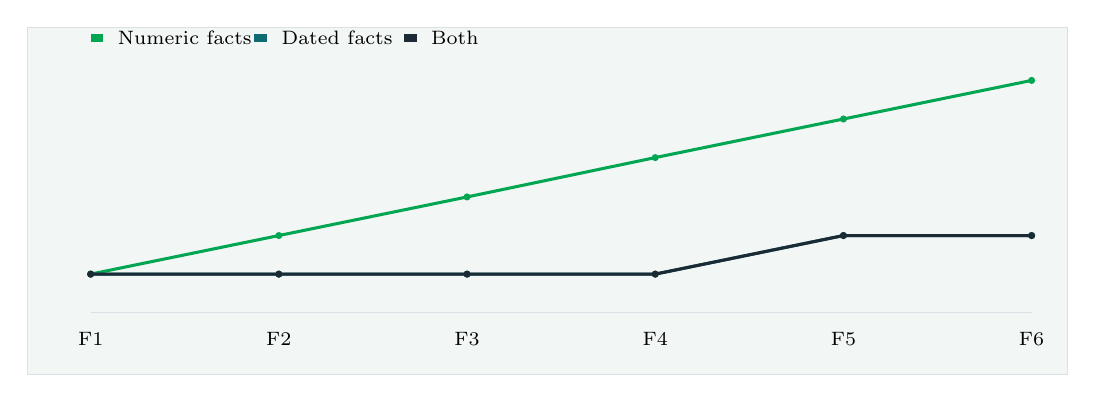
\begin{tikzpicture}[x=1cm,y=1cm]
\path[use as bounding box] (0,0) rectangle (13.20,4.40);
\fill[BOLight] (0,0) rectangle (13.20,4.40);
\draw[BOLine,line width=.35pt] (0,0) rectangle (13.20,4.40);
\draw[BOLine] (0.80,0.78) -- (12.75,0.78);
\draw[BOGreen,line width=1.1pt] (0.80,1.27) -- (3.19,1.76) -- (5.58,2.25) -- (7.97,2.75) -- (10.36,3.24) -- (12.75,3.73);
\fill[BOGreen] (0.80,1.27) circle (.045);
\fill[BOGreen] (3.19,1.76) circle (.045);
\fill[BOGreen] (5.58,2.25) circle (.045);
\fill[BOGreen] (7.97,2.75) circle (.045);
\fill[BOGreen] (10.36,3.24) circle (.045);
\fill[BOGreen] (12.75,3.73) circle (.045);
\draw[BOBlue,line width=1.1pt] (0.80,1.27) -- (3.19,1.27) -- (5.58,1.27) -- (7.97,1.27) -- (10.36,1.76) -- (12.75,1.76);
\fill[BOBlue] (0.80,1.27) circle (.045);
\fill[BOBlue] (3.19,1.27) circle (.045);
\fill[BOBlue] (5.58,1.27) circle (.045);
\fill[BOBlue] (7.97,1.27) circle (.045);
\fill[BOBlue] (10.36,1.76) circle (.045);
\fill[BOBlue] (12.75,1.76) circle (.045);
\draw[BONavy,line width=1.1pt] (0.80,1.27) -- (3.19,1.27) -- (5.58,1.27) -- (7.97,1.27) -- (10.36,1.76) -- (12.75,1.76);
\fill[BONavy] (0.80,1.27) circle (.045);
\fill[BONavy] (3.19,1.27) circle (.045);
\fill[BONavy] (5.58,1.27) circle (.045);
\fill[BONavy] (7.97,1.27) circle (.045);
\fill[BONavy] (10.36,1.76) circle (.045);
\fill[BONavy] (12.75,1.76) circle (.045);
\node[anchor=north,align=center,text width=1.8cm] at (0.80,0.66) {\scriptsize F1};
\node[anchor=north,align=center,text width=1.8cm] at (3.19,0.66) {\scriptsize F2};
\node[anchor=north,align=center,text width=1.8cm] at (5.58,0.66) {\scriptsize F3};
\node[anchor=north,align=center,text width=1.8cm] at (7.97,0.66) {\scriptsize F4};
\node[anchor=north,align=center,text width=1.8cm] at (10.36,0.66) {\scriptsize F5};
\node[anchor=north,align=center,text width=1.8cm] at (12.75,0.66) {\scriptsize F6};
\fill[BOGreen] (0.80,4.22) rectangle (0.96,4.32);
\node[anchor=west] at (1.02,4.27) {\scriptsize Numeric facts};
\fill[BOBlue] (2.88,4.22) rectangle (3.04,4.32);
\node[anchor=west] at (3.10,4.27) {\scriptsize Dated facts};
\fill[BONavy] (4.78,4.22) rectangle (4.94,4.32);
\node[anchor=west] at (5.00,4.27) {\scriptsize Both};
\end{tikzpicture}\par\vspace{2pt}
\vspace{1pt}\noindent\begin{minipage}[t]{0.56\linewidth}
{\footnotesize\color{BOText} Facts that combine dates and numbers are easier for a board reader to verify and compare across sources.}\par
\end{minipage}\hfill\begin{minipage}[t]{0.36\linewidth}
{\scriptsize\color{BOText}\begin{tabular}{p{31mm}>{\raggedleft\arraybackslash}p{18mm}}
\multicolumn{2}{l}{\textcolor{BOGreen}{\bfseries Visible readout}}\\[2pt]
F1 & \textbf{3}\\[1pt]
F2 & \textbf{4}\\[1pt]
F3 & \textbf{5}\\[1pt]
F4 & \textbf{6}\\[1pt]
F5 & \textbf{9}\\[1pt]
\end{tabular}}\par
\end{minipage}\par\vspace{1pt}
\vspace{4pt}{\footnotesize\color{BOText} Facts that combine dates and numbers are easier for a board reader to verify and compare across sources.}\par
{\scriptsize\color{BOMuted} Sources: science.osti.gov; energy.gov; iaea.org; iter.org.}\par

\clearpage
\label{chap:7}
\noindent\begin{tikzpicture}
\path[use as bounding box] (0,0) rectangle (\linewidth,54mm);
\clip (0,0) rectangle (\linewidth,54mm);
\node[anchor=north west,inner sep=0] at (0,54mm) {
\includegraphics[width=\linewidth]{assets/image-7.png}};
\end{tikzpicture}
\vspace{0pt}
\noindent
\begin{tikzpicture}
\fill[BOGreen] (0,0) rectangle (96mm,1.2pt);
\end{tikzpicture}\par\vspace{8pt}
{\Large\sffamily\bfseries\color{BONavy} Nuclear Fusion Commercialization Outlook and Strategic Implications should be managed as a staged strategic option, not a binary bet}\par\vspace{4pt}
{\sffamily\fontsize{15}{20}\selectfont\color{BOGreen} The CEO question is which moves are safe now and which should wait for stronger proof.}\par\vspace{9pt}
\begin{multicols}{2}
{\small Nuclear Fusion Commercialization Outlook and Strategic Implications is easier to misread when it is framed as a yes-or-no bet. The better reading separates near-term learning moves, option-building partnerships and commitments that would require stronger commercial proof.}\par
{\small The immediate management question is not whether the opportunity is exciting; it is whether budget, partner access or management attention should be committed now. Low-cost validation can start early, while larger capital commitments should wait for customer, cost, financing, regulatory or operating proof.}\par
{\small In capital terms, the current source base is useful but incomplete. A public source anchors this point: The Department of Energy has been a leader in fusion energy research since the 1950s and supports groundbreaking advances today. A quarterly review rhythm is more useful than a one-time verdict because the facts that matter will change as customers, regulators and suppliers move.}\par
{\small For Nuclear Fusion Commercialization Outlook and Strategic Implications should be managed as a staged strategic option, not., the executive question is practical: which commitments create learning without locking the company into a cost curve, customer promise or regulatory position that the facts cannot yet support.}\par
{\small For capital allocation, for Nuclear Fusion Commercialization Outlook and Strategic Implications should be managed as a staged strategic option, not., capital should move only when proof improves along the dimensions that change a business case: customer demand, cost position, financing availability, regulatory path and delivery capability. If those facts do not improve, larger exposure creates lock-in rather than conviction.}\par
{\small Operationally, for Nuclear Fusion Commercialization Outlook and Strategic Implications should be managed as a staged strategic option, not., the strongest public fact pattern is narrow but useful: The Department of Energy has been a leader in fusion energy research since the 1950s and supports groundbreaking advances today. It should shape the next customer, cost or partner question without being stretched into proof of commercial scale.}\par
\end{multicols}
\label{chap:7:end}

\clearpage
\label{chap:8}
\noindent\begin{tikzpicture}
\path[use as bounding box] (0,0) rectangle (\linewidth,54mm);
\clip (0,0) rectangle (\linewidth,54mm);
\node[anchor=north west,inner sep=0] at (0,54mm) {
\includegraphics[width=\linewidth]{assets/image-8.png}};
\end{tikzpicture}
\vspace{0pt}
\noindent
\begin{tikzpicture}
\fill[BOGreen] (0,0) rectangle (96mm,1.2pt);
\end{tikzpicture}\par\vspace{8pt}
{\Large\sffamily\bfseries\color{BONavy} Commercial readiness depends on bankability, deliverability and repeat customer proof}\par\vspace{4pt}
{\sffamily\fontsize{15}{20}\selectfont\color{BOGreen} Technical feasibility matters only when it changes customer value, cost position and execution confidence.}\par\vspace{9pt}
\begin{multicols}{2}
{\small For leadership teams, commercial readiness should be judged through customer adoption, cost structure, delivery cycle, service capability and financing availability. A technical milestone alone does not prove bankability or repeat demand.}\par
{\small Every major assumption needs a verifiable claim behind it: target customer, buying trigger, budget owner, substitute, use case and payback path. Where sourced evidence is missing, the claim should remain directional.}\par
{\small A more robust path is to build credible proof through pilots, partner diligence and third-party validation before moving into larger commitments.}\par
{\small For Commercial readiness depends on bankability, deliverability and repeat customer proof, the executive question is practical: which commitments create learning without locking the company into a cost curve, customer promise or regulatory position that the facts cannot yet support.}\par
{\small Operationally, for Commercial readiness depends on bankability, deliverability and repeat customer proof, capital should move only when proof improves along the dimensions that change a business case: customer demand, cost position, financing availability, regulatory path and delivery capability. If those facts do not improve, larger exposure creates lock-in rather than conviction.}\par
{\small For the board, for Commercial readiness depends on bankability, deliverability and repeat customer proof, the strongest public fact pattern is narrow but useful: The Department of Energy has been a leader in fusion energy research since the 1950s and supports groundbreaking advances today. It should shape the next customer, cost or partner question without being stretched into proof of commercial scale.}\par
\end{multicols}
\label{chap:8:end}

\clearpage
{\textcolor{BOGreen}{\scriptsize\bfseries EXHIBIT 13}}\par\vspace{4pt}
{\sffamily\fontsize{17}{21}\selectfont\color{BONavy} Strategic coverage balances market, cost, policy and execution proof}\par
{\small\color{BOText} Relative coverage on a five-point scale.}\par\vspace{6pt}
\noindent\fcolorbox{BOLine}{BOLight}{\begin{minipage}{0.96\linewidth}\vspace{4pt}{\scriptsize\begin{tabular}{p{38mm}>{\centering\arraybackslash}p{21mm}>{\centering\arraybackslash}p{21mm}>{\centering\arraybackslash}p{21mm}>{\centering\arraybackslash}p{21mm}}
 & {\bfseries Market} & {\bfseries Cost} & {\bfseries Policy} & {\bfseries Execution} \\
\hline
{\bfseries Fusion Commercialization Is} & \colorbox{BOGreen}{\textcolor{white}{\strut\hspace{5pt}5\hspace{5pt}}} & \colorbox{BOLight}{\textcolor{BOText}{\strut\hspace{5pt}2\hspace{5pt}}} & \colorbox{BOGreen}{\textcolor{white}{\strut\hspace{5pt}5\hspace{5pt}}} & \colorbox{BOGreen}{\textcolor{white}{\strut\hspace{5pt}5\hspace{5pt}}} \\
{\bfseries Fusion Faces High Cost Hurdles} & \colorbox{BOGreen}{\textcolor{white}{\strut\hspace{5pt}5\hspace{5pt}}} & \colorbox{BOGreen}{\textcolor{white}{\strut\hspace{5pt}5\hspace{5pt}}} & \colorbox{BOLight}{\textcolor{BOText}{\strut\hspace{5pt}2\hspace{5pt}}} & \colorbox{BOGreen}{\textcolor{white}{\strut\hspace{5pt}5\hspace{5pt}}} \\
{\bfseries Fusion Will Reshape Energy} & \colorbox{BOGreen}{\textcolor{white}{\strut\hspace{5pt}5\hspace{5pt}}} & \colorbox{BOGreen}{\textcolor{white}{\strut\hspace{5pt}5\hspace{5pt}}} & \colorbox{BOLight}{\textcolor{BOText}{\strut\hspace{5pt}1\hspace{5pt}}} & \colorbox{BOGreen}{\textcolor{white}{\strut\hspace{5pt}4\hspace{5pt}}} \\
{\bfseries Private Startups Are} & \colorbox{BOBlue}{\textcolor{white}{\strut\hspace{5pt}3\hspace{5pt}}} & \colorbox{BOLight}{\textcolor{BOText}{\strut\hspace{5pt}1\hspace{5pt}}} & \colorbox{BOGreen}{\textcolor{white}{\strut\hspace{5pt}5\hspace{5pt}}} & \colorbox{BOGreen}{\textcolor{white}{\strut\hspace{5pt}5\hspace{5pt}}} \\
{\bfseries Strategic Investments Should} & \colorbox{BOGreen}{\textcolor{white}{\strut\hspace{5pt}4\hspace{5pt}}} & \colorbox{BOLight}{\textcolor{BOText}{\strut\hspace{5pt}1\hspace{5pt}}} & \colorbox{BOBlue}{\textcolor{white}{\strut\hspace{5pt}3\hspace{5pt}}} & \colorbox{BOGreen}{\textcolor{white}{\strut\hspace{5pt}5\hspace{5pt}}} \\
\end{tabular}}\vspace{4pt}\end{minipage}}\par\vspace{2pt}
\vspace{1pt}\noindent\begin{minipage}[t]{0.56\linewidth}
{\footnotesize\color{BOText} A balanced executive view connects the market case with cost evidence, policy timing and execution constraints.}\par
\end{minipage}\hfill\begin{minipage}[t]{0.36\linewidth}
{\scriptsize\color{BOText}\begin{tabular}{p{31mm}>{\raggedleft\arraybackslash}p{18mm}}
\multicolumn{2}{l}{\textcolor{BOGreen}{\bfseries Matrix readout}}\\[2pt]
Fusion & \textbf{5 / 2}\\[1pt]
Fusion Faces High & \textbf{5 / 5}\\[1pt]
Fusion Will Reshape & \textbf{5 / 5}\\[1pt]
Private Startups Are & \textbf{3 / 1}\\[1pt]
\end{tabular}}\par
\end{minipage}\par\vspace{1pt}
\vspace{4pt}{\footnotesize\color{BOText} A balanced executive view connects the market case with cost evidence, policy timing and execution constraints.}\par
{\scriptsize\color{BOMuted} Sources: public references and report analysis.}\par
\vspace{9pt}\textcolor{BOLine}{\rule{\linewidth}{0.3pt}}\vspace{8pt}
{\textcolor{BOGreen}{\scriptsize\bfseries EXHIBIT 14}}\par\vspace{4pt}
{\sffamily\fontsize{17}{21}\selectfont\color{BONavy} Triangulation is strongest where domains, facts and years overlap}\par
{\small\color{BOText} Composite view of public domains, extracted facts and explicit dates.}\par\vspace{6pt}
\noindent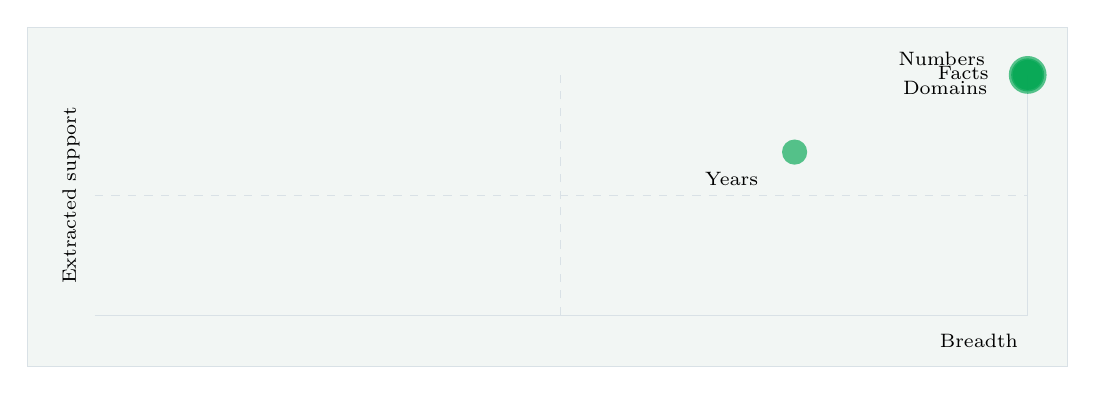
\begin{tikzpicture}[x=1cm,y=1cm]
\path[use as bounding box] (0,0) rectangle (13.20,4.30);
\fill[BOLight] (0,0) rectangle (13.20,4.30);
\draw[BOLine,line width=.35pt] (0,0) rectangle (13.20,4.30);
\draw[BOLine] (0.85,0.65) -- (12.70,0.65) -- (12.70,3.70);
\draw[BOLine,dashed] (0.85,2.17) -- (12.70,2.17);
\draw[BOLine,dashed] (6.77,0.65) -- (6.77,3.70);
\fill[BOGreen,opacity=.65] (12.70,3.70) circle (0.21);
\node[anchor=east,align=right,text width=2.10cm] at (12.31,3.54) {\scriptsize Domains};
\fill[BOGreen,opacity=.65] (12.70,3.70) circle (0.19);
\node[anchor=east,align=right,text width=2.10cm] at (12.33,3.73) {\scriptsize Facts};
\fill[BOGreen,opacity=.65] (9.74,2.72) circle (0.16);
\node[anchor=east,align=right,text width=2.10cm] at (9.40,2.38) {\scriptsize Years};
\fill[BOGreen,opacity=.65] (12.70,3.70) circle (0.24);
\node[anchor=east,align=right,text width=2.10cm] at (12.28,3.91) {\scriptsize Numbers};
\node[anchor=north east] at (12.70,0.53) {\scriptsize Breadth};
\node[anchor=center,rotate=90] at (0.55,2.17) {\scriptsize Extracted support};
\end{tikzpicture}\par\vspace{2pt}
\vspace{1pt}\noindent\begin{minipage}[t]{0.56\linewidth}
{\footnotesize\color{BOText} The commercial conclusion becomes more credible when multiple source domains, fact types and dated milestones point in the same direction.}\par
\end{minipage}\hfill\begin{minipage}[t]{0.36\linewidth}
{\scriptsize\color{BOText}\begin{tabular}{p{31mm}>{\raggedleft\arraybackslash}p{18mm}}
\multicolumn{2}{l}{\textcolor{BOGreen}{\bfseries Position}}\\[2pt]
Domains & \textbf{100 / 100}\\[1pt]
Facts & \textbf{100 / 100}\\[1pt]
Years & \textbf{75 / 68}\\[1pt]
Numbers & \textbf{100 / 100}\\[1pt]
\end{tabular}}\par
\end{minipage}\par\vspace{1pt}
\vspace{4pt}{\footnotesize\color{BOText} The commercial conclusion becomes more credible when multiple source domains, fact types and dated milestones point in the same direction.}\par
{\scriptsize\color{BOMuted} Sources: science.osti.gov; energy.gov; iaea.org; iter.org.}\par

\clearpage
\noindent
\begin{tikzpicture}
\fill[BOGreen] (0,0) rectangle (46mm,1.2pt);
\end{tikzpicture}\par\vspace{8pt}
{\sffamily\fontsize{22}{27}\selectfont\color{BONavy} Research basis and limitations}\par\vspace{9pt}
\begin{minipage}[t]{0.47\linewidth}
{\sffamily\fontsize{15}{20}\selectfont\color{BOGreen} Public materials support a strategic view, not a transaction recommendation.}\par\vspace{7pt}
{\footnotesize\color{BOText} This report has been prepared for strategy discussion and executive decision support. It is not investment, legal, tax, audit or valuation advice. Market estimates, forecasts and scenarios are directional and should be independently validated before they are used for investment, financing, transaction, regulatory or operational decisions. Forward-looking views may change as technology, policy, financing, regulation, competition, supply chains and macro conditions evolve. Recipients should perform their own diligence and treat this report as one input into a broader decision process.}\par
\end{minipage}\hfill\begin{minipage}[t]{0.46\linewidth}
{\textcolor{BOGreen}{\scriptsize\bfseries PUBLIC MATERIALS REFERENCED}}\par\vspace{5pt}
\begin{tabularx}{\linewidth}{p{8mm}Y}
\textcolor{BOGreen}{\bfseries 01} & {\scriptsize Osti} \\[4pt]
\textcolor{BOGreen}{\bfseries 02} & {\scriptsize Energy} \\[4pt]
\textcolor{BOGreen}{\bfseries 03} & {\scriptsize Iaea} \\[4pt]
\textcolor{BOGreen}{\bfseries 04} & {\scriptsize Iter} \\[4pt]
\textcolor{BOGreen}{\bfseries 05} & {\scriptsize Nationalacademies} \\[4pt]
\textcolor{BOGreen}{\bfseries 06} & {\scriptsize Fusionindustryassociation} \\[4pt]
\textcolor{BOGreen}{\bfseries 07} & {\scriptsize Llnl} \\[4pt]
\end{tabularx}
\end{minipage}\par\vspace{12pt}
\fcolorbox{BOLine}{BOLight}{\begin{minipage}{0.96\linewidth}\vspace{5pt}\begin{tabularx}{\linewidth}{Y Y Y}
{\textcolor{BOGreen}{\scriptsize\bfseries USE}}\par{\scriptsize Use the report to clarify timing, partner selection, capital exposure and the next management decision.} & {\textcolor{BOGreen}{\scriptsize\bfseries DO NOT USE}}\par{\scriptsize Do not treat directional market views as a substitute for transaction diligence, technical verification or legal advice.} & {\textcolor{BOGreen}{\scriptsize\bfseries UPDATE TRIGGER}}\par{\scriptsize Refresh the view when public milestones, cost curves, regulation, financing or customer commitments materially change.} \\
\end{tabularx}\vspace{5pt}\end{minipage}}

\clearpage
\noindent
\begin{tikzpicture}
\fill[BOGreen] (0,0) rectangle (38mm,1.2pt);
\end{tikzpicture}\par\vspace{8pt}
{\sffamily\fontsize{24}{30}\selectfont\color{BONavy} About BlueOcean}\par\vspace{10pt}
\begin{minipage}[t]{0.44\linewidth}
{\sffamily\fontsize{16}{22}\selectfont\color{BOGreen} Research is most useful when it changes a management decision.}\par\vspace{8pt}
{\footnotesize\color{BOText} BlueOcean prepares decision-focused research for executives who need to separate credible evidence from market noise, translate technology shifts into commercial implications and stage commitments around proof.}\par\vspace{7pt}
{\footnotesize\color{BOMuted} This report draws on Osti, Energy, Iaea, Iter, Nationalacademies, Fusionindustryassociation, Llnl.}\par
\vspace{10pt}\fcolorbox{BOLine}{BOLight}{\begin{minipage}{0.90\linewidth}\vspace{5pt}{\scriptsize\color{BOText} The work is designed for CEOs and leadership teams who need a concise view of what changes now, what waits for stronger proof and which external facts would change the answer.}\vspace{5pt}\end{minipage}}
\end{minipage}\hfill\begin{minipage}[t]{0.48\linewidth}
{\textcolor{BOGreen}{\scriptsize\bfseries HOW BLUEOCEAN SUPPORTS EXECUTIVE TEAMS}}\par\vspace{5pt}
\begin{tabularx}{\linewidth}{p{8mm}Y}
\textcolor{BOGreen}{\bfseries 01} & {\scriptsize\bfseries Strategy research}\par{\scriptsize Decision-focused market, technology and competitive research for senior leadership.} \\[6pt]
\textcolor{BOGreen}{\bfseries 02} & {\scriptsize\bfseries Evidence synthesis}\par{\scriptsize Structured comparison of public materials, company claims, policy signals and market data.} \\[6pt]
\textcolor{BOGreen}{\bfseries 03} & {\scriptsize\bfseries Executive output}\par{\scriptsize Reader-ready reports, exhibits and board materials designed for fast management discussion.} \\[6pt]
\textcolor{BOGreen}{\bfseries 04} & {\scriptsize\bfseries Quality control}\par{\scriptsize Source retention, language cleanup and layout checks before publication.} \\[6pt]
\end{tabularx}\vspace{6pt}
\begin{tabularx}{\linewidth}{p{31mm}Y}
{\small\bfseries This report was prepared by a strategic research team with expertise in energy}\par{\scriptsize\color{BOGreen} Research synthesis team} & {\footnotesize Responsible for evidence checks, executive synthesis and report QA.} \\[7pt]
\end{tabularx}
\end{minipage}

\clearpage
\thispagestyle{empty}
\AddToShipoutPictureBG*{\AtPageLowerLeft{
\includegraphics[width=\paperwidth,height=\paperheight]{assets/cover-ai.png}}}

\vspace*{\fill}
\begin{flushright}
{\sffamily\bfseries\Large\color{white} BlueOcean}\hspace*{3mm}
\end{flushright}
\vspace*{8mm}

\end{document}
